% ----------------------------------------------------------------------------
% Multi-Object Tracking for Sports Analytics (Player and Ball Tracking)
% IEEE conference format (IEEEtran).
%
% Compile:  pdflatex FINAL_REPORT.tex   (run twice so references resolve)
%           or upload FINAL_REPORT_IEEE_overleaf.zip to Overleaf.
%
% This file is GENERATED by scripts/make_latex_report.py from
% docs/latex/FINAL_REPORT.template.tex and results/metrics/. Edit the template
% (text) or re-run the experiments (numbers), then run the script again.
% Figures are expected in the folder figures/ next to this file.
% ----------------------------------------------------------------------------
\documentclass[conference]{IEEEtran}
\IEEEoverridecommandlockouts
\usepackage[T1]{fontenc}
\usepackage{cite}
\usepackage{amsmath,amssymb}
\usepackage{graphicx}
\usepackage{booktabs}
\usepackage{array}
\usepackage{adjustbox}
\usepackage{url}
\graphicspath{{figures/}}

\begin{document}

\title{Multi-Object Tracking for Sports Analytics:\\
Player and Ball Tracking with YOLO11n, ByteTrack, a Kalman Filter and Motion-Based Ball Flights}

% TODO before submitting: replace the bracketed fields with your details. For more
% authors, add further \and \IEEEauthorblockN{...}\IEEEauthorblockA{...} blocks.
\author{\IEEEauthorblockN{Yaswanth}
\IEEEauthorblockA{\textit{[Department]} \\
\textit{[Institution]}\\
{[City, Country]} \\
{[e-mail address]}}}

\maketitle

\begin{abstract}
This paper presents a lightweight tracking-by-detection system that tracks soccer
players and the ball in monocular video on a CPU. A COCO-pretrained YOLO11n
detector finds people and the ball in a single pass per frame, ByteTrack assigns
persistent player identities, and a constant-velocity Kalman filter tracks the
ball and predicts its position through short detection gaps, labelling every
predicted position as such. When the ball is struck and the detector loses the
motion-blurred ball, camera-motion-compensated moving blobs linked into fast,
smooth flights that must start at the ball let the tracker follow it. The proposed player tracker is compared with SORT and
OC-SORT on identical cached detections from six test sequences of SportsMOT and
UVY-Track (2,950 frames), with hyper-parameters chosen on a separate sequence. The
ball tracker is compared with detection-only output on 13 sequences of UVY-Track
and InFactory (2,402 frames with a visible ball). On SportsMOT, ByteTrack gives
the fewest identity switches (51, against 60 for SORT and 106 for OC-SORT) and the
highest recall (95.9\%), while tuned SORT reaches a higher HOTA (65.9 against
62.6) because it outputs fewer boxes on people the benchmark does not annotate.
On the partially labelled UVY-Track clips ByteTrack has the best OWTA (56.8). The
proposed ball tracker raises ball precision from 66.4\% to 70.0\%, recall from
34.8\% to 36.4\% and F1 from 45.7\% to 47.9\% over detection alone and merges 175
correct track segments into 44; on a free kick its motion flights raise ball
recall from 91.1\% to 99.4\%. The detector accounts for 64\% of the processing time
and is the main limit on accuracy. The proposed method is therefore not uniformly better
than the baselines; the paper reports where it helps, where it does not, and why.
\end{abstract}

\begin{IEEEkeywords}
multi-object tracking, sports analytics, soccer, ball tracking, YOLO, ByteTrack,
SORT, OC-SORT, Kalman filter, HOTA, frame differencing
\end{IEEEkeywords}

% =============================================================================
\section{Introduction}
% =============================================================================
Broadcast and amateur sports video is increasingly analysed automatically for
coaching, scouting, officiating support and fan engagement. Almost every such
analysis (distance covered, possession, heatmaps, pass maps, tactical shape)
starts from the same two signals: where every player is over time, with a stable
identity, and where the ball is. Producing these signals from a single camera is
a multi-object tracking (MOT) problem with sport-specific difficulties: players
of one team look alike, so appearance gives little help in telling them apart;
motion is fast and non-linear, with frequent occlusion in duels and set pieces;
broadcast cameras pan and zoom, so image motion mixes camera and player motion;
and the ball is tiny (often 5--20 pixels), blurred, frequently hidden, and moves
much faster than any player.

This work builds a complete, lightweight tracking-by-detection system for this
task and evaluates it quantitatively. It runs on a CPU, uses only pretrained
models, and is organised so that each stage (detector, player tracker, ball
tracker) can be replaced and measured independently. The contributions are:
\begin{itemize}
\item a working pipeline that turns a soccer video into an annotated video, a
per-frame tracking table and a run summary, in which ball positions predicted by
a motion model are always distinguished from detected ones;
\item a controlled comparison of ByteTrack with SORT and OC-SORT in which all
trackers replay identical detections and are tuned with the same budget on a
sequence disjoint from the test data;
\item an evaluation on three public datasets with different annotation schemes,
including an analysis of how partially labelled data invalidates
false-positive-based metrics;
\item a ball-tracking evaluation that reports the benefit and the cost of motion
prediction separately;
\item a motion-based extension of the ball tracker that follows a struck,
motion-blurred ball which the generic detector misses, by linking
camera-motion-compensated moving blobs into physically plausible flights that must
start at the ball.
\end{itemize}

% =============================================================================
\section{Related Work}
% =============================================================================
\textbf{Tracking by detection.} Modern MOT systems detect objects in every frame
and associate detections over time. SORT~\cite{sort} showed that a Kalman
filter~\cite{kalman} for motion prediction plus Hungarian
assignment~\cite{hungarian} on bounding-box overlap is a strong and very fast
baseline. DeepSORT~\cite{deepsort} added an appearance embedding to reduce
identity switches through occlusion. ByteTrack~\cite{bytetrack} observed that
discarding low-confidence detections throws away true objects that are occluded
or blurred, and introduced a second association stage that matches the remaining
tracks to low-confidence boxes. OC-SORT~\cite{ocsort} kept the simplicity of SORT
but corrected the error accumulated by the Kalman filter during occlusion with an
observation-centric re-update, and added a motion-direction consistency term.
BoT-SORT~\cite{botsort} combined ByteTrack with camera-motion compensation and
re-identification.

\textbf{Tracking in sports.} Manafifard \emph{et al.}~\cite{survey} survey player
tracking in soccer video. SoccerNet-Tracking~\cite{soccernet} and
SportsMOT~\cite{sportsmot} are the main public benchmarks; SportsMOT emphasises
fast, variable-speed motion and similar appearance and identifies association,
rather than detection, as the key difficulty in sports. SoccerTrack~\cite{soccertrack}
and TeamTrack~\cite{teamtrack} provide full-pitch fisheye and drone footage.
UVY-Track~\cite{uvy,uvypaper} targets unconstrained user-generated sports video
rather than broadcast footage.

\textbf{Ball detection and tracking.} The ball is a small-object problem.
DeepBall~\cite{deepball} and TrackNet~\cite{tracknet} use specialised fully
convolutional networks; TrackNet stacks consecutive frames so that the network
can exploit motion. Slicing-aided inference~\cite{sahi} improves small-object
recall for generic detectors by running them on overlapping tiles. A common
lightweight alternative, used here, is to keep a generic detector and add a
single-target motion model that rejects implausible candidates and bridges short
gaps. Classical broadcast ball trackers also use motion directly: trajectory-based
methods~\cite{yu2006} generate many ball candidates and keep only the candidate
chains whose motion is plausible for a ball. This work adds such a step for the
ball in flight.

\textbf{Detectors and metrics.} The YOLO family~\cite{yolo} performs detection in
a single network pass; this work uses the COCO-pretrained~\cite{coco} YOLO11 nano
model~\cite{yolo11}. CLEAR-MOT~\cite{clear} defines MOTA, which is dominated by
detection errors. IDF1~\cite{idf1} measures identity preservation.
HOTA~\cite{hota} balances detection and association explicitly and is the primary
metric of SportsMOT. OWTA~\cite{owta} removes the false-positive penalty for
data in which not every object is labelled.

% =============================================================================
\section{Problem Statement, Research Gap and Objectives}
% =============================================================================
\textbf{Problem.} Given a monocular sports video, produce for every frame (i) a
bounding box and a persistent identity for every player and (ii) the position of
the ball, stating explicitly whether that position was detected in the frame or
predicted by a motion model; and quantify detection quality, identity
preservation, ball coverage and processing speed against baseline trackers under
identical conditions.

\textbf{Gap.} Published sports trackers are usually evaluated with detectors
fine-tuned on the benchmark and on GPUs; less is reported about how the classic
trackers behave with a generic, lightweight, CPU-friendly detector, which is the
realistic setting for a low-cost system. Players and the ball are also different
tracking problems: players are many similar objects that need global assignment,
whereas the ball is one tiny, frequently missed object, and benchmarks such as
SportsMOT annotate players only. Finally, when a system interpolates the ball
position, results frequently do not say which positions were observed and which
were inferred. This motivates a hybrid design, a multi-object tracker for players
and a dedicated single-target Kalman tracker for the ball, evaluated separately.

\textbf{Objectives.} (1) Detect players and the ball with a lightweight
pretrained detector. (2) Track players with persistent identities using
ByteTrack. (3) Track the ball with a Kalman filter that bridges short detection
gaps without presenting a predicted position as a detection, and that follows the
ball in flight when the detector loses it. (4) Export an
annotated video, a per-frame table and a run summary. (5) Compare with SORT and
OC-SORT on identical detections, frames and ground truth. (6) Evaluate on three
public datasets with standard metrics. (7) Make every result reproducible.

% =============================================================================
\section{Proposed System}
% =============================================================================
\begin{figure*}[t]
\centering
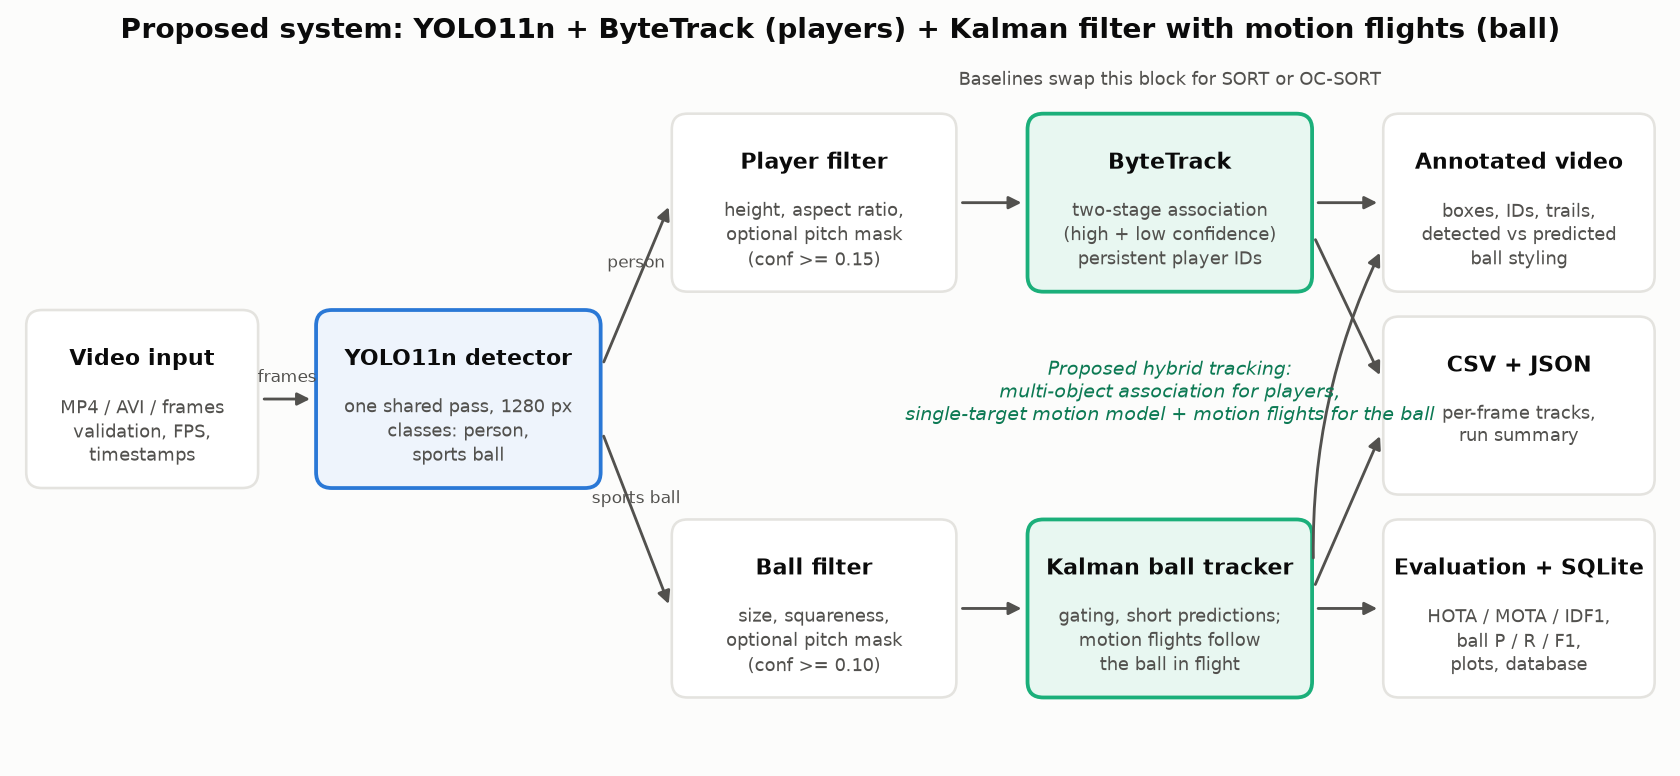
\includegraphics[width=0.92\textwidth]{fig_architecture.png}
\caption{Architecture of the proposed system. One YOLO11n pass per frame serves
players and ball; ByteTrack tracks the players and a Kalman filter, extended with
motion-based flights, tracks the ball. For the baselines only the player-tracker block is replaced by SORT or
OC-SORT.}
\label{fig:architecture}
\end{figure*}

\subsection{Overview}
Fig.~\ref{fig:architecture} shows the pipeline. Each frame is decoded and passed
once through the detector, which reports the COCO classes \emph{person} and
\emph{sports ball}. Inexpensive geometric filters remove implausible boxes.
Player boxes go to the multi-object tracker and ball candidates to the ball
tracker, which also receives motion-based ball flights computed from the frames. The tracked objects are drawn on the frame and streamed to a
comma-separated file; a summary is written at the end. Players are many similar
objects that need global assignment, whereas the ball is a single small object
that is often missed, so the two are tracked by different algorithms: this
combination is the proposed hybrid.

\subsection{Detection and Filtering}
YOLO11n (COCO weights, about 2.6 million parameters) is run at an input size of
1280 pixels with a non-maximum-suppression threshold of 0.5. Detections of
\emph{person} with confidence at least 0.15 and of \emph{sports ball} with
confidence at least 0.10 are kept. The thresholds are deliberately low because
the trackers, not the detector threshold, decide what to trust. Player boxes must
be between 12 pixels and 60\% of the frame height tall with a height-to-width
ratio between 0.8 and 6. Ball boxes must be 2--80 pixels in size and roughly
square (aspect ratio at most 2). Sharing one network pass between the two classes
halves the detection cost compared with two passes.

\subsection{Player Tracking}
SORT, OC-SORT and ByteTrack share one structure: each track is predicted with a
Kalman filter, a cost matrix of intersection-over-union (IoU) between predicted
boxes and detections is solved with the Hungarian algorithm, matched tracks are
updated, unmatched detections start new tracks, and tracks that stay unmatched
for a number of frames are deleted. They differ in how detections are used.
SORT has a single association stage. OC-SORT uses only detections above a
confidence threshold and adds an observation-centric re-update after occlusion
and a direction-consistency term. ByteTrack first associates high-confidence
detections and then uses the low-confidence ones to keep the remaining tracks
alive.

ByteTrack is the proposed player tracker because, in sports, players are often
partly occluded or motion-blurred, which lowers detector confidence without the
player disappearing; ByteTrack is designed to keep such tracks alive instead of
dropping them, which should reduce identity switches and fragmentation. It needs
no appearance model, so it remains fast on a CPU and is not confused by identical
kits.

\subsection{Ball Tracking}
Ball candidates come from the same detector pass. The ball tracker is a
constant-velocity Kalman filter with state
$\mathbf{x}=[x,\,y,\,\dot{x},\,\dot{y}]^{\top}$ and a time step of one frame:
\begin{equation}
\mathbf{x}_{k}=\mathbf{F}\mathbf{x}_{k-1}+\mathbf{w}_{k},\qquad
\mathbf{z}_{k}=\mathbf{H}\mathbf{x}_{k}+\mathbf{v}_{k},
\label{eq:kalman}
\end{equation}
\begin{equation}
\mathbf{F}=\begin{bmatrix}1&0&1&0\\0&1&0&1\\0&0&1&0\\0&0&0&1\end{bmatrix},\qquad
\mathbf{H}=\begin{bmatrix}1&0&0&0\\0&1&0&0\end{bmatrix},
\label{eq:matrices}
\end{equation}
where $\mathbf{w}_{k}$ models an unknown acceleration with a standard deviation
of 4 pixels per frame squared and $\mathbf{v}_{k}$ a measurement error with a
standard deviation of 4 pixels. Four rules turn the filter of
(\ref{eq:kalman})--(\ref{eq:matrices}) into a tracker.

\emph{Gating.} A candidate is accepted only if its distance $d_{i}$ to the
predicted position is within a gate
\begin{equation}
g_{k}=\min\left(g_{0}+m_{k}\,\Delta g,\; g_{\max}\right),
\label{eq:gate}
\end{equation}
with $g_{0}=80$ pixels, $\Delta g=20$ pixels, $g_{\max}=160$ pixels and $m_{k}$ the
number of consecutive frames without an accepted detection. Among several candidates with confidence
$c_{i}$ the one that maximises
\begin{equation}
s_{i}=c_{i}\left(1-\frac{d_{i}}{g_{k}}\right)
\label{eq:score}
\end{equation}
is taken. This rejects false balls elsewhere in the image.

\emph{Confirmation.} A new track needs a detection with confidence at least 0.3
and is reported only after two detections, which suppresses one-frame false
positives; weaker detections can only extend an existing track.

\emph{Prediction through gaps.} With no accepted candidate, the filter coasts for
up to 6 frames (0.2~s) and the output is labelled \emph{predicted}. It does not
coast right after a sudden jump of the measured position (a kick), because the new
velocity is unknown.

\emph{Re-acquisition.} A detection with confidence at least 0.5 outside the gate
restarts the track after three missed frames, which handles long passes and
camera cuts.

Predicted positions are kept distinct from end to end: a different marker and the
text ``ball (predicted)'' in the video, a \emph{predicted} status with an empty
confidence in the exported table, separate counts in the run summary, and
separate columns in every ball table of this paper.

\subsection{Ball in Flight: Motion Flights}
A struck ball is motion-blurred into a pale streak and the COCO detector almost
never fires on it, while extrapolating the last velocity through a kick is wrong
(Section~\ref{sec:ballresults}). Three components follow the ball in flight.

\emph{Motion candidates.} The two previous frames are aligned to the current one
with a similarity transform estimated from ORB features~\cite{orb} with
RANSAC~\cite{ransac}, which cancels camera pan and zoom. A pixel is moving if it
differs from both aligned frames (three-frame differencing using only past frames,
so the ghost at the ball's old position is suppressed). Bright, low-saturation
moving pixels are grouped into components, and small, compact components are
candidates. They are noisy by design: boots, socks and shirt numbers also move.

\emph{Flights.} Candidates are linked frame to frame under a constant-velocity
model. A chain counts as a flight while it has at least six points, a median
speed of at least 8 pixels per frame and a smooth path, with a median change of
velocity of at most $\max(4, 0.3\,\bar{v})$ pixels for median speed $\bar{v}$;
this is re-checked every frame. Limbs swing back and forth and running players are
slower, so they rarely qualify.

\emph{Adoption.} A flight is used as the ball only if it was launched from the
ball: its first velocity $\mathbf{v}_{0}$, run backwards from its first point
$\mathbf{p}_{0}$ at frame $t_{0}$ to the frame $t_{s}$ at which the detector last
saw the ball at $\mathbf{b}$, must satisfy
\begin{equation}
\left\lVert \mathbf{p}_{0}-\mathbf{v}_{0}\,(t_{0}-t_{s})-\mathbf{b}\right\rVert \le 35~\text{pixels}.
\label{eq:launch}
\end{equation}
Anchors are detector sightings only, so a wrong flight can never anchor the next
one. A confident detection inside the gate prevents a new flight from being
adopted, while a flight already being followed outranks single detections, which
during a shot are often the goalkeeper's glove. When the followed flight ends
abruptly (net, save, bounce) the ball is reported lost rather than extrapolated. A
flight is confirmed only after six frames, so the pipeline holds its output eight
frames and fills in the first frames of the flight. Flight positions are
observations, reported as detected with the class name \emph{ball (motion)} and no
detector confidence.

% =============================================================================
\section{Datasets}
\label{sec:datasets}
% =============================================================================
Three public datasets are used (Table~\ref{tab:datasets}). Each has its own
loader and annotations from different datasets are never mixed. The annotation
format of every dataset was inspected on the downloaded files before its loader
was written; UVY-Track, for example, is a multi-object-tracking text format with
a class column, not a YOLO format. Only the required sequences were downloaded by
reading the remote archives selectively (0.73~GB instead of about 11~GB).
Table~\ref{tab:sequences} lists the evaluated sequences: 4{,}850 frames in
total (1{,}831 SportsMOT, 1{,}569 UVY-Track, 1{,}450 InFactory).

\begin{table*}[t]
\caption{Datasets and How They Are Used}
\label{tab:datasets}
\centering
\footnotesize
\begin{tabular}{@{}p{2.6cm}p{4.2cm}p{4.9cm}p{4.6cm}@{}}
\toprule
 & SportsMOT~\cite{sportsmot} & UVY-Track~\cite{uvy,uvypaper} & InFactory Soccer Ball Tracking~\cite{infactory} \\
\midrule
Footage & Professional broadcast (football, basketball, volleyball) & User-generated online sports videos, seven sports & Professional soccer broadcast \\
Annotation format & MOT Challenge text & MOT-style text with a class column & YOLO text, one file per frame \\
Annotated objects & Players on the pitch only & Player, goalkeeper, referee, sports ball, goal, camera & Ball only, plus frames marked ``ball not visible'' \\
Persistent identities & Players & People and ball & None \\
Role in this work & Player tracking (tuning and test) & Player tracking and ball detection/tracking (test) & Ball detection (test) \\
Subset used & 4 football sequences of the validation split & 3 soccer sequences & 10 clips (884 frames with a visible ball, 566 without) \\
\bottomrule
\end{tabular}
\end{table*}

\begin{table}[t]
\caption{Evaluated Sequences}
\label{tab:sequences}
\centering
\footnotesize
\setlength{\tabcolsep}{3pt}
\begin{adjustbox}{max width=\columnwidth}
\begin{tabular}{@{}llcrrr@{}}
\toprule
Dataset & Sequence & Role & Frames & Tracks & Ball fr. \\
\midrule
SportsMOT & \texttt{v\_2QhNRucNC7E\_c017} & dev & 450 & 21 & -- \\
SportsMOT & \texttt{v\_dw7LOz17Omg\_c067} & test & 450 & 22 & -- \\
SportsMOT & \texttt{v\_G-vNjfx1GGc\_c008} & test & 480 & 20 & -- \\
SportsMOT & \texttt{v\_i2\_L4qquVg0\_c007} & test & 451 & 21 & -- \\
UVY-Track & \texttt{soccer\_V04} & test & 219 & 19 & 168 \\
UVY-Track & \texttt{soccer\_V01} & test & 750 & 6 & 750 \\
UVY-Track & \texttt{soccer\_V03} & test & 600 & 5 & 600 \\
InFactory & 10 clips & test & 1{,}450 & -- & 884 \\
\bottomrule
\end{tabular}
\end{adjustbox}
\end{table}

\textbf{Tuning versus testing.} One SportsMOT sequence
(\texttt{v\_2QhNRucNC7E\_c017}) is the only data used to choose tracker
hyper-parameters. It comes from a different source video than every test sequence
and is never included in test averages. Nothing is tuned on UVY-Track or
InFactory.

\textbf{Two properties of the data matter for the results.} First, SportsMOT
labels only the players, so referees, coaches and perimeter staff detected by a
generic \emph{person} detector count as false positives. Second, UVY-Track labels
only part of the people: in the fan-filmed penalty-kick clips \texttt{soccer\_V01}
and \texttt{soccer\_V03} the four to six people involved in the kick have boxes,
while dozens of visible photographers, staff and other players do not. Metrics
that count false positives are therefore not valid error measures on UVY-Track.
Its ball boxes are also loose, about twice the size of the detector boxes
($20\times26$ against $12\times11$ pixels on \texttt{soccer\_V03}), so an IoU of
0.5 is rarely reached even by a perfectly centred detection. InFactory has no ball
identities, so only detection-type metrics are reported for it.

% =============================================================================
\section{Experimental Setup}
% =============================================================================
\subsection{Baselines and Fairness Protocol}
Three player-tracking configurations are compared: YOLO11n + SORT, YOLO11n +
OC-SORT, and the proposed YOLO11n + ByteTrack with the Kalman ball tracker. All
three tracker implementations come from the open-source \texttt{trackers}
package~\cite{trackers} and share one update interface, so no tracker was
re-implemented. The protocol is as follows.
\begin{itemize}
\item The detector output is computed once per sequence and cached; every
tracker replays exactly the same detections on the same frames and is scored
against the same ground truth with the same evaluator.
\item Hyper-parameters are chosen per tracker on the dev sequence with the same
48-point grid (track buffer in \{30, 60\} frames, frames before confirmation in
\{1, 3\}, minimum IoU in \{0.1, 0.2, 0.3\}, confidence threshold in
\{0.3, 0.4, 0.5, 0.6\}) and the same rule: highest HOTA, ties broken by IDF1.
Table~\ref{tab:params} lists the selected values.
\item Results are also reported for one shared, untuned parameter set, so that
the effect of tuning is visible.
\end{itemize}

\begin{table}[t]
\caption{Tracker Parameters (n/a: Parameter Not Used by the Tracker)}
\label{tab:params}
\centering
\footnotesize
\setlength{\tabcolsep}{3pt}
\begin{adjustbox}{max width=\columnwidth}
\begin{tabular}{@{}lccccc@{}}
\toprule
 & Buffer & Confirm & Min. & New-track & High-conf. \\
Parameter set & (frames) & (frames) & IoU & threshold & threshold \\
\midrule
Shared default & 30 & 3 & 0.1 & 0.5 & 0.5 \\
\midrule
SORT, tuned & 30 & 1 & 0.3 & 0.6 & n/a \\
OC-SORT, tuned & 60 & 1 & 0.3 & n/a & 0.3 \\
ByteTrack (proposed), tuned & 30 & 1 & 0.2 & 0.5 & 0.5 \\
\bottomrule
\end{tabular}
\end{adjustbox}
\end{table}

For the ball, four outputs are compared on identical candidates: the most
confident candidate of each frame with no temporal reasoning (\emph{detection
only}); the positions that the Kalman tracker reports from a detection, as an
ablation; the Kalman tracker on detector candidates alone (detected and predicted
positions, \emph{YOLO only}), as an ablation without motion flights; and the full
proposed tracker with motion flights, exactly as in the application. The Kalman
part runs with its default configuration and is not tuned on any evaluated
sequence. The motion-flight rules, however, were developed while inspecting the
UVY-Track clip \texttt{soccer\_V04}, and a first full run on InFactory exposed two
failure modes (a camera cut and a fast object passing the ball) that led to two
further rules, so the ball results of the proposed method are not from fully
held-out data. A further clip, \texttt{soccer\_V02}, never used for any decision,
was checked qualitatively.

\subsection{Metrics}
Player tracking is scored with the evaluation module of the \texttt{trackers}
package~\cite{trackers}, a re-implementation designed to match
TrackEval~\cite{trackeval}, the reference evaluator of MOTChallenge and
SportsMOT. HOTA~\cite{hota} is the primary metric,
\begin{equation}
\mathrm{HOTA}_{\alpha}=\sqrt{\mathrm{DetA}_{\alpha}\cdot\mathrm{AssA}_{\alpha}},
\label{eq:hota}
\end{equation}
averaged over localisation thresholds $\alpha$ from 0.05 to 0.95, where DetA and
AssA are the detection and association accuracies. MOTA~\cite{clear} and
IDF1~\cite{idf1} are
\begin{equation}
\mathrm{MOTA}=1-\frac{\mathrm{FN}+\mathrm{FP}+\mathrm{IDSW}}{\mathrm{GT}},
\label{eq:mota}
\end{equation}
\begin{equation}
\mathrm{IDF1}=\frac{2\,\mathrm{IDTP}}{2\,\mathrm{IDTP}+\mathrm{IDFP}+\mathrm{IDFN}},
\label{eq:idf1}
\end{equation}
computed at an IoU threshold of 0.5. Also reported are identity switches (IDSW),
false positives (FP), false negatives (FN), fragmentations (Frag) and mostly
tracked targets (MT). For the partially labelled UVY-Track data the
false-positive penalty is removed by using~\cite{owta}
\begin{equation}
\mathrm{OWTA}_{\alpha}=\sqrt{\mathrm{DetRe}_{\alpha}\cdot\mathrm{AssA}_{\alpha}},
\label{eq:owta}
\end{equation}
together with the detection recall DetRe.

Ball and detector metrics are computed with an evaluator written for this
project. It is unit-tested on hand-computed cases but is not an official
benchmark tool. A method outputs at most one ball position per frame. An output
is correct under the \emph{distance} criterion if its centre lies within one ball
diameter of the true centre, and under the \emph{IoU} criterion if its IoU with a
ground-truth box is at least 0.5. Precision, recall (the visible-ball recall) and
F1 follow from the per-frame outcomes. AP@0.5 is the average precision of all
ball candidates ranked by confidence; with one class it equals mAP@0.5. Coverage
is the share of labelled frames with any output. Continuity is described by the
number and mean length of correctly tracked segments inside runs of visible-ball
frames. Ball identity switches are reported only for UVY-Track, which has ball
identities.

\subsection{Implementation and Hardware}
All experiments ran on an Apple M1 CPU (8 physical / 8 logical cores), 8.0~GB RAM, no GPU used (device: cpu), macOS, Python~3.14.6, PyTorch~2.15.0 with 7 threads, Ultralytics~8.4.198, \texttt{trackers}~2.6.1, \texttt{supervision}~0.31.3 and OpenCV~5.0.0. The system has 121 automated tests,
including an end-to-end test of the full pipeline. All results are reproduced by
one command in the project repository\footnote{\url{https://github.com/YaswanthKumar814/Multi-Object-Tracking-for-Sports-Analytics-}};
the evaluated sequences and frame ranges are fixed in a manifest file. The
numbers are computed on small subsets with a generic detector and are not
comparable with leaderboard entries.

% =============================================================================
\section{Results}
% =============================================================================
\subsection{Player Detection}
Table~\ref{tab:detection} compares the detector output with the ground-truth
player boxes before any tracking. Recall is above 92\% on the SportsMOT test
sequences. Precision is limited by real people who are not annotated, and on
UVY-Track it cannot be interpreted at all for the reason given in Section~\ref{sec:datasets}.

\begin{table}[t]
\caption{Player Detection with YOLO11n (Confidence $\geq 0.5$, IoU $\geq 0.5$)}
\label{tab:detection}
\centering
\footnotesize
\setlength{\tabcolsep}{4pt}
\begin{adjustbox}{max width=\columnwidth}
\begin{tabular}{@{}lccrrrr@{}}
\toprule
Dataset & Role & Seq. & Prec. & Rec. & F1 & AP@0.5 \\
\midrule
SportsMOT & dev & 1 & 92.4 & 89.3 & 90.8 & 90.1 \\
SportsMOT & test & 3 & 81.3 & 92.2 & 86.4 & 88.9 \\
UVY-Track & test & 3 & 49.6$^{\dagger}$ & 70.8 & 58.3$^{\dagger}$ & 57.4$^{\dagger}$ \\
\bottomrule
\multicolumn{7}{@{}l}{$^{\dagger}$Not meaningful: only part of the people are labelled.} \\
\end{tabular}
\end{adjustbox}
\end{table}

\subsection{Player Tracking on SportsMOT}
Table~\ref{tab:sportsmot} and Fig.~\ref{fig:tracking} give the results on the
three SportsMOT test sequences (1,381 frames, 16,360 ground-truth boxes).

\begin{table*}[t]
\caption{Player Tracking on the SportsMOT Test Sequences with Identical YOLO11n
Detections. Best Value per Column and Parameter Set in Bold (Lower Is Better for
IDSW, FP, FN and Frag)}
\label{tab:sportsmot}
\centering
\footnotesize
\setlength{\tabcolsep}{5pt}
\begin{adjustbox}{max width=\textwidth}
\begin{tabular}{@{}lrrrrrrrrrrrr@{}}
\toprule
Method & HOTA & DetA & AssA & MOTA & IDF1 & IDSW & FP & FN & Frag & MT & Prec. & Rec. \\
\midrule
\multicolumn{13}{l}{\textit{Parameters tuned per tracker on the dev sequence}} \\
YOLO11n + SORT & \textbf{65.9} & \textbf{64.8} & \textbf{67.0} & \textbf{64.9} & \textbf{70.6} & 60 & \textbf{4{,}898} & 784 & \textbf{158} & 59 & \textbf{76.1} & 95.2 \\
YOLO11n + OC-SORT & 59.3 & 60.6 & 58.0 & 55.3 & 61.2 & 106 & 6{,}382 & 817 & 230 & 61 & 70.9 & 95.0 \\
YOLO11n + ByteTrack (proposed) & 62.6 & 59.4 & 66.1 & 52.6 & 66.8 & \textbf{51} & 7{,}029 & \textbf{670} & 168 & \textbf{62} & 69.1 & \textbf{95.9} \\
\midrule
\multicolumn{13}{l}{\textit{One shared, untuned parameter set (project defaults)}} \\
YOLO11n + SORT & \textbf{64.1} & 59.5 & \textbf{69.0} & 52.9 & 68.6 & 44 & 6{,}975 & \textbf{687} & \textbf{174} & \textbf{61} & 69.2 & \textbf{95.8} \\
YOLO11n + OC-SORT & 63.5 & \textbf{67.4} & 59.9 & \textbf{71.1} & \textbf{69.4} & 61 & \textbf{2{,}629} & 2{,}030 & 259 & 52 & \textbf{84.5} & 87.6 \\
YOLO11n + ByteTrack (proposed) & 63.3 & 59.4 & 67.4 & 52.9 & 67.8 & \textbf{43} & 6{,}963 & 696 & \textbf{174} & \textbf{61} & 69.2 & 95.7 \\
\bottomrule
\end{tabular}
\end{adjustbox}
\end{table*}

\begin{figure*}[t]
\centering
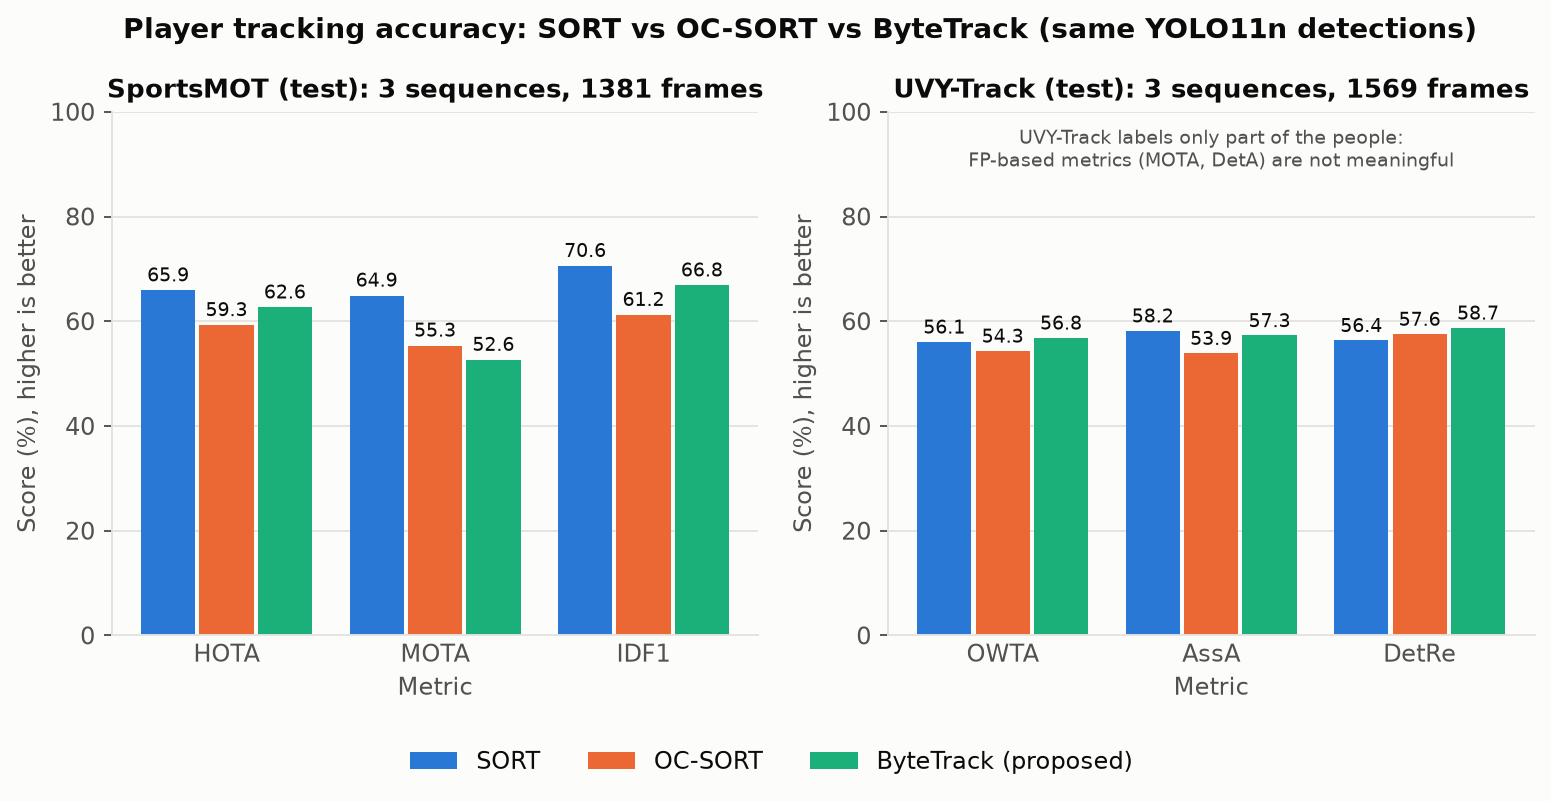
\includegraphics[width=0.86\textwidth]{fig_tracking_accuracy.png}
\caption{Tracking accuracy of the three trackers with tuned parameters. Left:
HOTA, MOTA and IDF1 on SportsMOT. Right: OWTA, AssA and detection recall on the
partially labelled UVY-Track.}
\label{fig:tracking}
\end{figure*}

\emph{Identity stability.} ByteTrack has the fewest identity switches (51), the
fewest missed boxes (670 false negatives, recall 95.9\%) and the most mostly
tracked players. OC-SORT has about twice as many switches (106) and the most
fragmented tracks (Fig.~\ref{fig:idsw}).

\emph{Overall accuracy.} Tuned SORT has the best HOTA (65.9), MOTA (64.9) and
IDF1 (70.6). ByteTrack is second on HOTA (62.6) and IDF1 (66.8). Its association
accuracy is within 0.9 points of SORT (AssA 66.1 against 67.0); the gap comes
from detection accuracy, because ByteTrack outputs 2,131 more false-positive
boxes.

\emph{Explanation.} The second association stage of ByteTrack keeps tracks alive
with low-confidence boxes. With a detector trained on the benchmark those boxes
are occluded players. With a generic detector on SportsMOT, many of them are
unannotated people at the edge of the pitch, so the mechanism that lowers the
number of misses also raises the number of false positives: 1,912 of the 2,131
extra false positives come from the single sequence with staff along the
perimeter boards. In addition, the SORT implementation used here already allows
any detection, including a low-confidence one, to match an existing track, so the
practical difference between the two trackers is smaller than in the original
papers; the tuned SORT settings (new tracks only above a confidence of 0.6,
IoU at least 0.3) simply start fewer tracks on bystanders.

\emph{Effect of tuning.} With one shared, untuned parameter set (lower half of
Table~\ref{tab:sportsmot}) the three trackers are within 0.8 HOTA points of each
other. ByteTrack again has the fewest identity switches (43). OC-SORT then has
the best MOTA (71.1) because it discards every box below a confidence of 0.5,
which removes many false positives but costs about 8 points of recall. On the dev
sequence itself ByteTrack was best on HOTA, MOTA, IDF1 and identity switches, but
this is not an independent result. The selected parameters did not transfer
equally well: the dev sequence contains few unannotated people, so a low
confidence threshold looked best for OC-SORT there and then hurt it on the test
sequences. Fig.~\ref{fig:tuning} shows the sensitivity of each tracker to its
parameters. Tuning on a single sequence is a limitation of this study.

\begin{figure}[t]
\centering
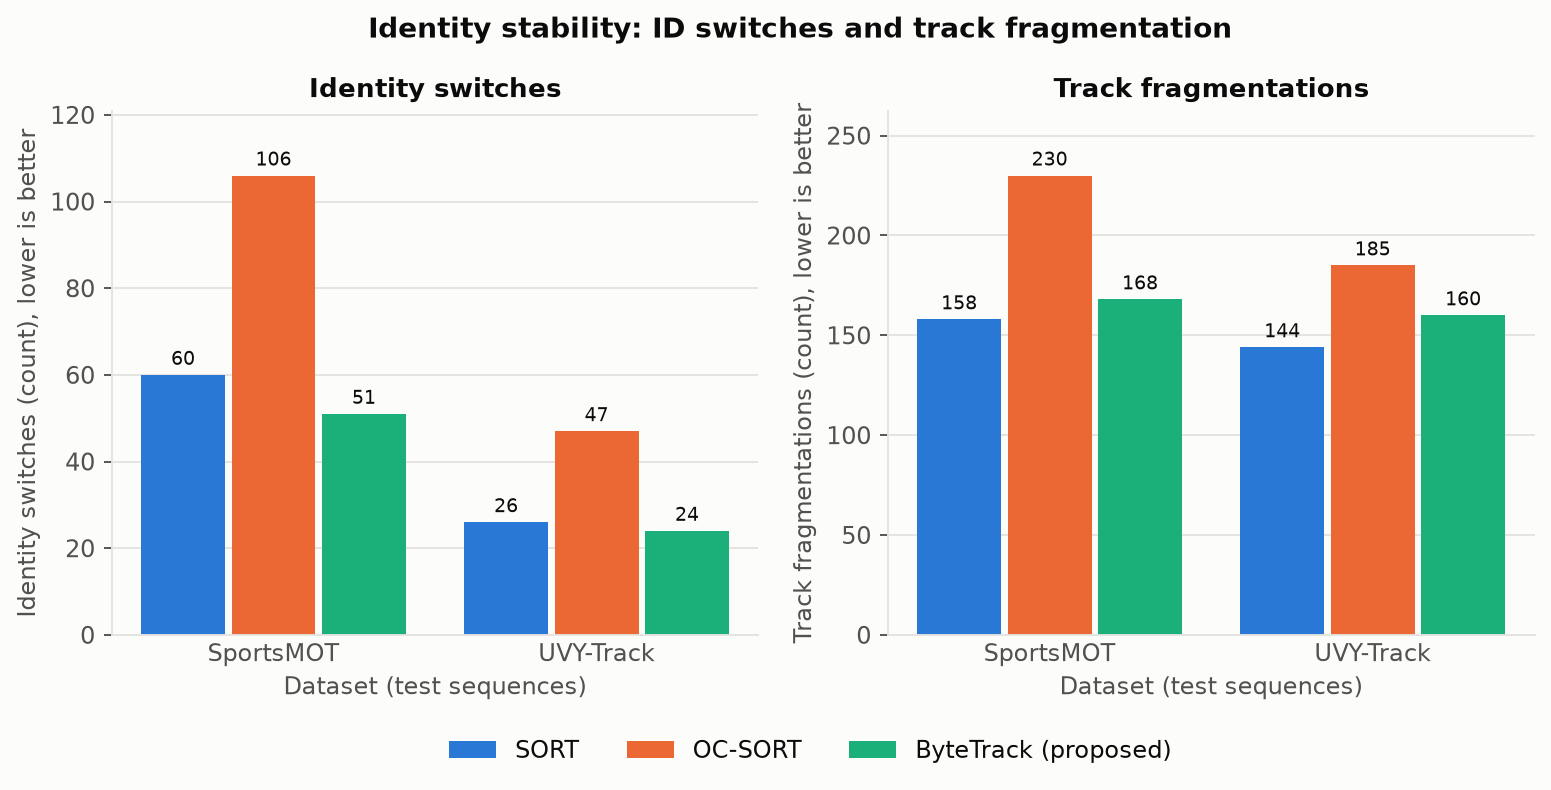
\includegraphics[width=\columnwidth]{fig_idsw_frag.png}
\caption{Identity switches and track fragmentations on the test sequences of
both datasets (lower is better).}
\label{fig:idsw}
\end{figure}

\begin{figure}[t]
\centering
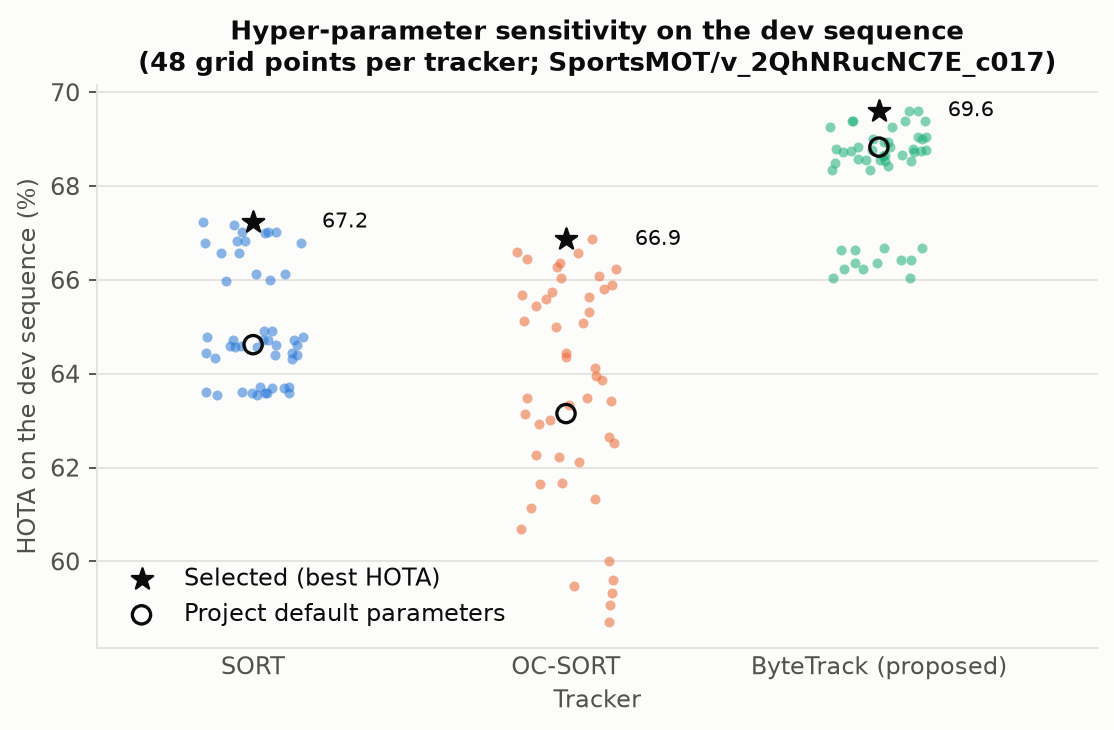
\includegraphics[width=0.9\columnwidth]{fig_tuning.png}
\caption{HOTA on the dev sequence for the 48 grid points of each tracker. Star:
selected setting. Circle: shared default setting.}
\label{fig:tuning}
\end{figure}

\subsection{Player Tracking on UVY-Track}
Table~\ref{tab:uvy} reports the metrics that remain valid when only part of the
people are labelled. On these the trackers are close. ByteTrack has the best OWTA
(56.8), the highest detection recall (58.7), the fewest identity switches (24)
and the fewest missed boxes; SORT has a marginally higher AssA and the fewest
fragmentations; OC-SORT has almost twice as many identity switches (47). For
completeness, MOTA on this dataset is negative for every tracker (between
$-32$ and $-93$), which reflects the unlabelled people and not tracker errors.
The low-resolution clip \texttt{soccer\_V01} ($636\times360$ pixels, people about
35 pixels tall) is difficult for all three trackers, with an OWTA of about 30.

\begin{table}[t]
\caption{Player Tracking on the UVY-Track Test Sequences (1,569 Frames, Tuned
Parameters). Only Metrics That Do Not Count False Positives Are Shown}
\label{tab:uvy}
\centering
\footnotesize
\setlength{\tabcolsep}{3.5pt}
\begin{adjustbox}{max width=\columnwidth}
\begin{tabular}{@{}lrrrrrrr@{}}
\toprule
Tracker & OWTA & DetRe & AssA & IDSW & Frag & MT & FN \\
\midrule
SORT & 56.1 & 56.4 & \textbf{58.2} & 26 & \textbf{144} & \textbf{16} & 2{,}524 \\
OC-SORT & 54.3 & 57.6 & 53.9 & 47 & 185 & \textbf{16} & 2{,}363 \\
ByteTrack (proposed) & \textbf{56.8} & \textbf{58.7} & 57.3 & \textbf{24} & 160 & \textbf{16} & \textbf{2{,}232} \\
\bottomrule
\end{tabular}
\end{adjustbox}
\end{table}

\subsection{Ball Detection and Tracking}
\label{sec:ballresults}
Table~\ref{tab:ball} summarises the ball results on 13 sequences (3,019 labelled
frames, 2,402 with a visible ball); Fig.~\ref{fig:prf} shows precision, recall
and F1.

\begin{table*}[t]
\caption{Ball Results: Detection Only Versus the Kalman Ball Tracker With and
Without Motion Flights on Identical Candidates. AP@0.5 Is Computed over All Detector Candidates. Coverage Is the
Share of Labelled Frames with an Output. Frames: Detected, Predicted, No Output. Segments: Number and Mean Length in Frames}
\label{tab:ball}
\centering
\footnotesize
\setlength{\tabcolsep}{3.5pt}
\begin{adjustbox}{max width=\textwidth}
\begin{tabular}{@{}llrrrrrrrrrrrrr@{}}
\toprule
 & & \multicolumn{3}{c}{Distance criterion (\%)} & \multicolumn{3}{c}{IoU $\geq 0.5$ (\%)} & AP@0.5 & Cover. & \multicolumn{3}{c}{Frames} & \multicolumn{2}{c}{Correct segments} \\
\cmidrule(lr){3-5}\cmidrule(lr){6-8}\cmidrule(lr){11-13}\cmidrule(lr){14-15}
Data & Method & Prec. & Rec. & F1 & Prec. & Rec. & F1 & (\%) & (\%) & Det. & Pred. & None & No. & Mean len. \\
\midrule
UVY-Track & Detection only & 62.6 & 35.1 & 45.0 & 24.8 & 13.9 & 17.8 & 12.0 & 54.3 & 852 & 0 & 717 & 102 & 5.2 \\
UVY-Track & Kalman, detected only & 67.0 & 28.1 & 39.6 & 34.2 & 14.4 & 20.2 & -- & 40.6 & 637 & 0 & 932 & 43 & 9.9 \\
UVY-Track & Kalman (YOLO only) & 65.6 & 35.2 & 45.8 & 27.8 & 14.9 & 19.4 & -- & 51.9 & 637 & 177 & 755 & 10 & 53.4 \\
UVY-Track & Kalman + motion (proposed) & 64.2 & 36.1 & 46.2 & 28.1 & 15.8 & 20.2 & -- & 54.4 & 672 & 182 & 715 & 11 & 49.8 \\
\midrule
InFactory & Detection only & 74.5 & 34.4 & 47.1 & 66.9 & 30.9 & 42.3 & 26.0 & 28.1 & 408 & 0 & 1{,}042 & 73 & 4.2 \\
InFactory & Kalman, detected only & 92.5 & 27.8 & 42.8 & 80.1 & 24.1 & 37.0 & -- & 18.3 & 266 & 0 & 1{,}184 & 50 & 4.9 \\
InFactory & Kalman (YOLO only) & 82.5 & 36.9 & 51.0 & 63.5 & 28.4 & 39.2 & -- & 27.2 & 266 & 129 & 1{,}055 & 33 & 9.9 \\
InFactory & Kalman + motion (proposed) & 82.5 & 36.9 & 51.0 & 63.5 & 28.4 & 39.2 & -- & 27.2 & 266 & 129 & 1{,}055 & 33 & 9.9 \\
\midrule
All (13 seq.) & Detection only & 66.4 & 34.8 & 45.7 & 38.4 & 20.1 & 26.4 & 16.3 & 41.7 & 1{,}260 & 0 & 1{,}759 & 175 & 4.8 \\
All (13 seq.) & Kalman, detected only & 74.5 & 28.0 & 40.7 & 47.7 & 17.9 & 26.1 & -- & 29.9 & 903 & 0 & 2{,}116 & 93 & 7.2 \\
All (13 seq.) & Kalman (YOLO only) & 71.1 & 35.8 & 47.6 & 39.5 & 19.9 & 26.4 & -- & 40.0 & 903 & 306 & 1{,}810 & 43 & 20.0 \\
All (13 seq.) & Kalman + motion (proposed) & 70.0 & 36.4 & 47.9 & 39.3 & 20.4 & 26.9 & -- & 41.4 & 938 & 311 & 1{,}770 & 44 & 19.9 \\
\bottomrule
\end{tabular}
\end{adjustbox}
\end{table*}

\begin{figure*}[t]
\centering
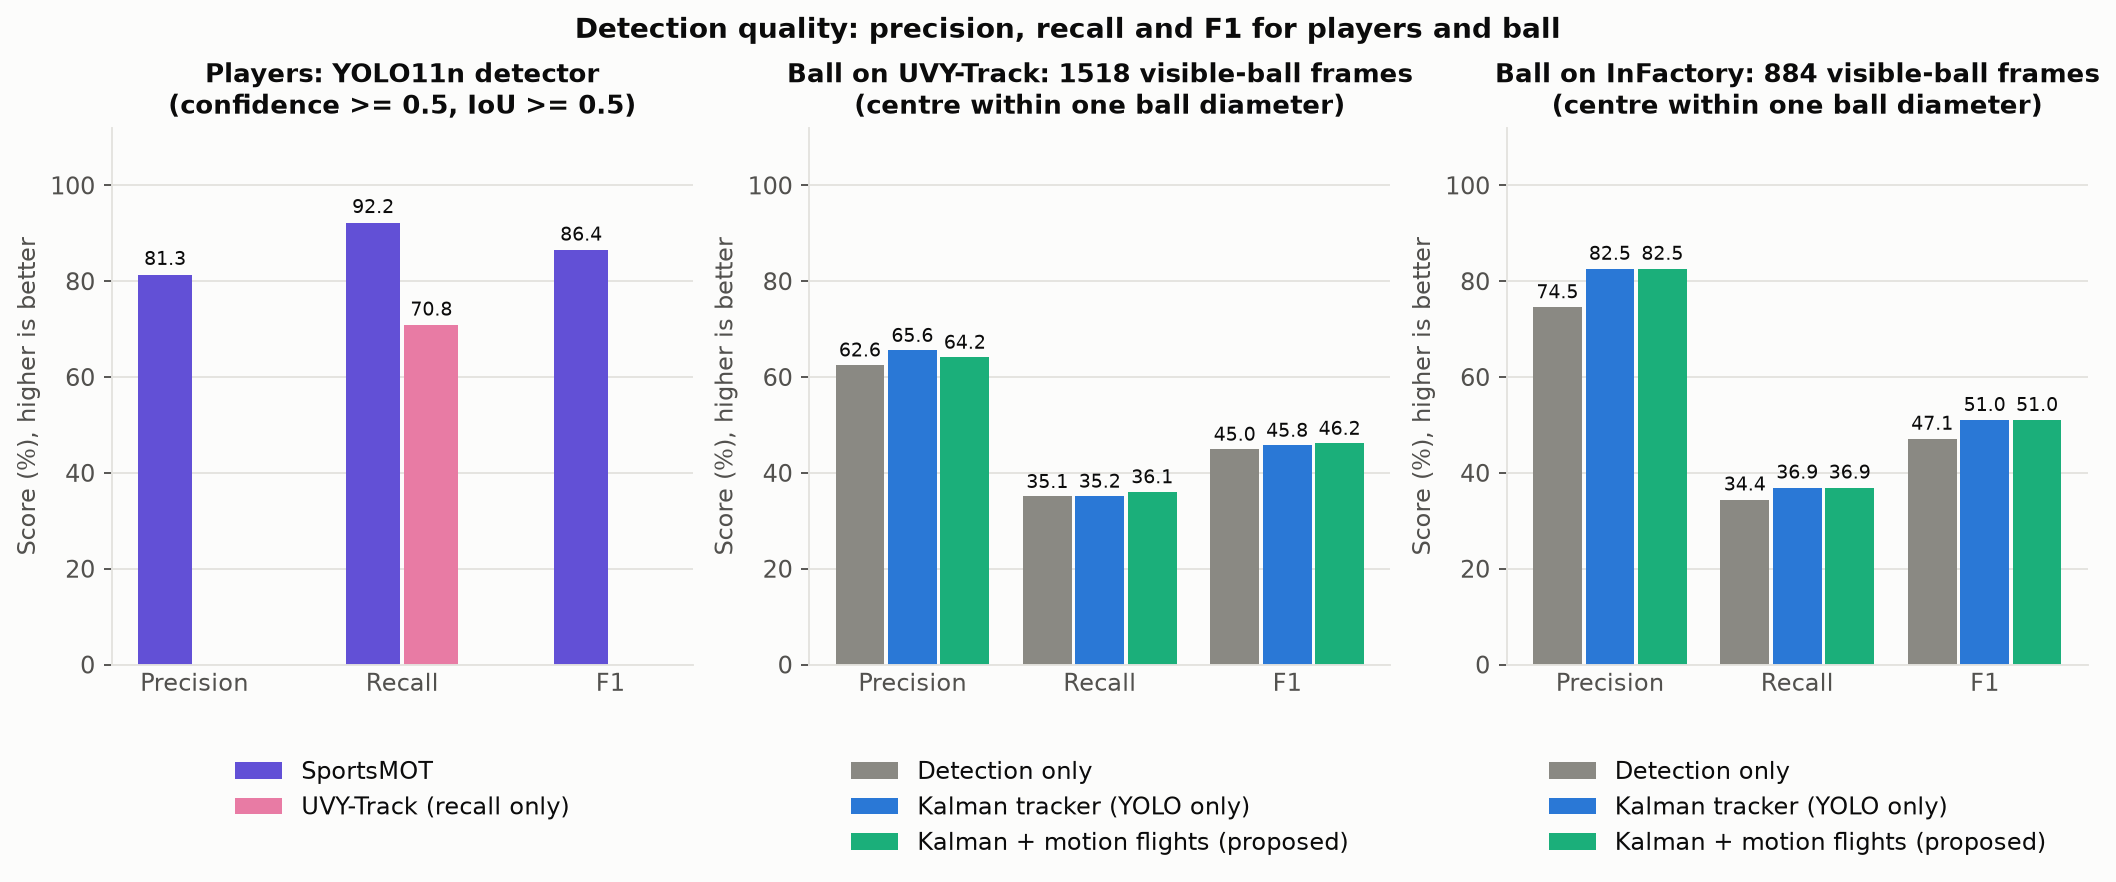
\includegraphics[width=\textwidth]{fig_detection_prf.png}
\caption{Precision, recall and F1. Left: player detection. Centre and right: the
ball on UVY-Track and on InFactory: detection only, the Kalman tracker on detector
candidates alone, and the proposed tracker with motion flights (distance criterion).}
\label{fig:prf}
\end{figure*}

\emph{The detector is the bottleneck.} The COCO \emph{sports ball} class finds
the ball in only about a third of the frames in which it is visible (recall
34.8\%; AP@0.5 of 16.3\% over all candidates). When it does respond to the ball
it is accurate: correct outputs lie about 2 pixels from the true centre.

\emph{Effect of the Kalman tracker.} Over detection alone, precision rises from
66.4\% to 71.1\%, recall from 34.8\% to 35.8\% and F1 from 45.7\% to 47.6\% under
the distance criterion, and F1 improves on both datasets. The tracker is
deliberately conservative (a confidence of at least 0.3 to start a track, a capped
gate, at most six coasted frames and none right after a kick). A looser earlier
version reached a higher recall (43.3\%) and F1 (49.3\%), but only 42.6\% of its
predicted positions were correct; the current version trades some recall for
positions that can be trusted. The ball track also becomes far more continuous:
with the proposed tracker 175 short correct segments merge into 44 and their mean
length grows from 4.8 to 19.9 frames. It recovers 249 visible-ball frames that
detection alone misses and loses 212 that detection alone had (the first
detection of each track, which is held back for confirmation, weak detections
that may not start a track, and detections outside the gate). On UVY-Track, the
only dataset with ball identities, the track identity changes four times.

\emph{Effect of motion flights.} On top of the Kalman tracker, recall rises from
35.8\% to 36.4\% and F1 from 47.6\% to 47.9\%. Flights fire only where the ball is
struck and visible in flight: on every InFactory clip and on two of the three
UVY-Track clips the output is identical to the Kalman tracker. On the free kick of
\texttt{soccer\_V04} the Kalman tracker loses the ball when it is struck (recall
91.1\%), whereas with motion flights the shot is followed from the boot into the
net (recall 99.4\%, Fig.~\ref{fig:balltraj}). Precision there falls from 97.5\% to
84.8\%, but all 24 outputs counted as false lie in frames in which the annotators
marked no ball (the most blurred part of the flight and the ball inside the net);
inspection shows these positions on the ball.

Table~\ref{tab:ballpred} separates detected and predicted outputs. Detected
positions accepted by the tracker are more precise than raw detections (73.2\%
against 66.4\%), because gating and confirmation reject isolated false balls.
Predicted positions are correct 60.1\% of the time: they are right when the ball
rolls or is briefly occluded and wrong when it changes direction during the gap,
because the filter extrapolates the last velocity. This is the reason for
reporting predicted positions separately.

\begin{table}[t]
\caption{Proposed Ball Tracker: Precision of Detected and of Predicted Positions
(Distance Criterion)}
\label{tab:ballpred}
\centering
\footnotesize
\begin{adjustbox}{max width=\columnwidth}
\begin{tabular}{@{}lrrrr@{}}
\toprule
 & \multicolumn{2}{c}{Detected} & \multicolumn{2}{c}{Predicted} \\
\cmidrule(lr){2-3}\cmidrule(lr){4-5}
Data & Frames & Prec. (\%) & Frames & Prec. (\%) \\
\midrule
UVY-Track & 672 & 65.6 & 182 & 58.8 \\
InFactory & 266 & 92.5 & 129 & 62.0 \\
All & 938 & 73.2 & 311 & 60.1 \\
\bottomrule
\end{tabular}
\end{adjustbox}
\end{table}

\emph{Strict localisation.} Under the IoU criterion F1 barely changes (26.4\% to
26.9\%), because a predicted box is rarely within an IoU of 0.5 of a ball that
is about 15 pixels wide. On UVY-Track the IoU-based numbers are low for every
method because of the loose ground-truth boxes described in Section~\ref{sec:datasets}; the
distance criterion is the meaningful one there.

\emph{Per-sequence behaviour is uneven.} Against detection only, F1 improves on
five sequences (for example from 45.6\% to 78.7\% on \texttt{71125020}), stays at
zero on three clips in which the detector never finds the ball, and decreases on
five (for example from 51.5\% to 47.5\% on \texttt{soccer\_V03}, and on
\texttt{7d503a7a}, where the track follows something other than the ball). Fig.~\ref{fig:ballstatus} shows the share of detected, predicted and
lost frames per sequence.

\begin{figure}[t]
\centering
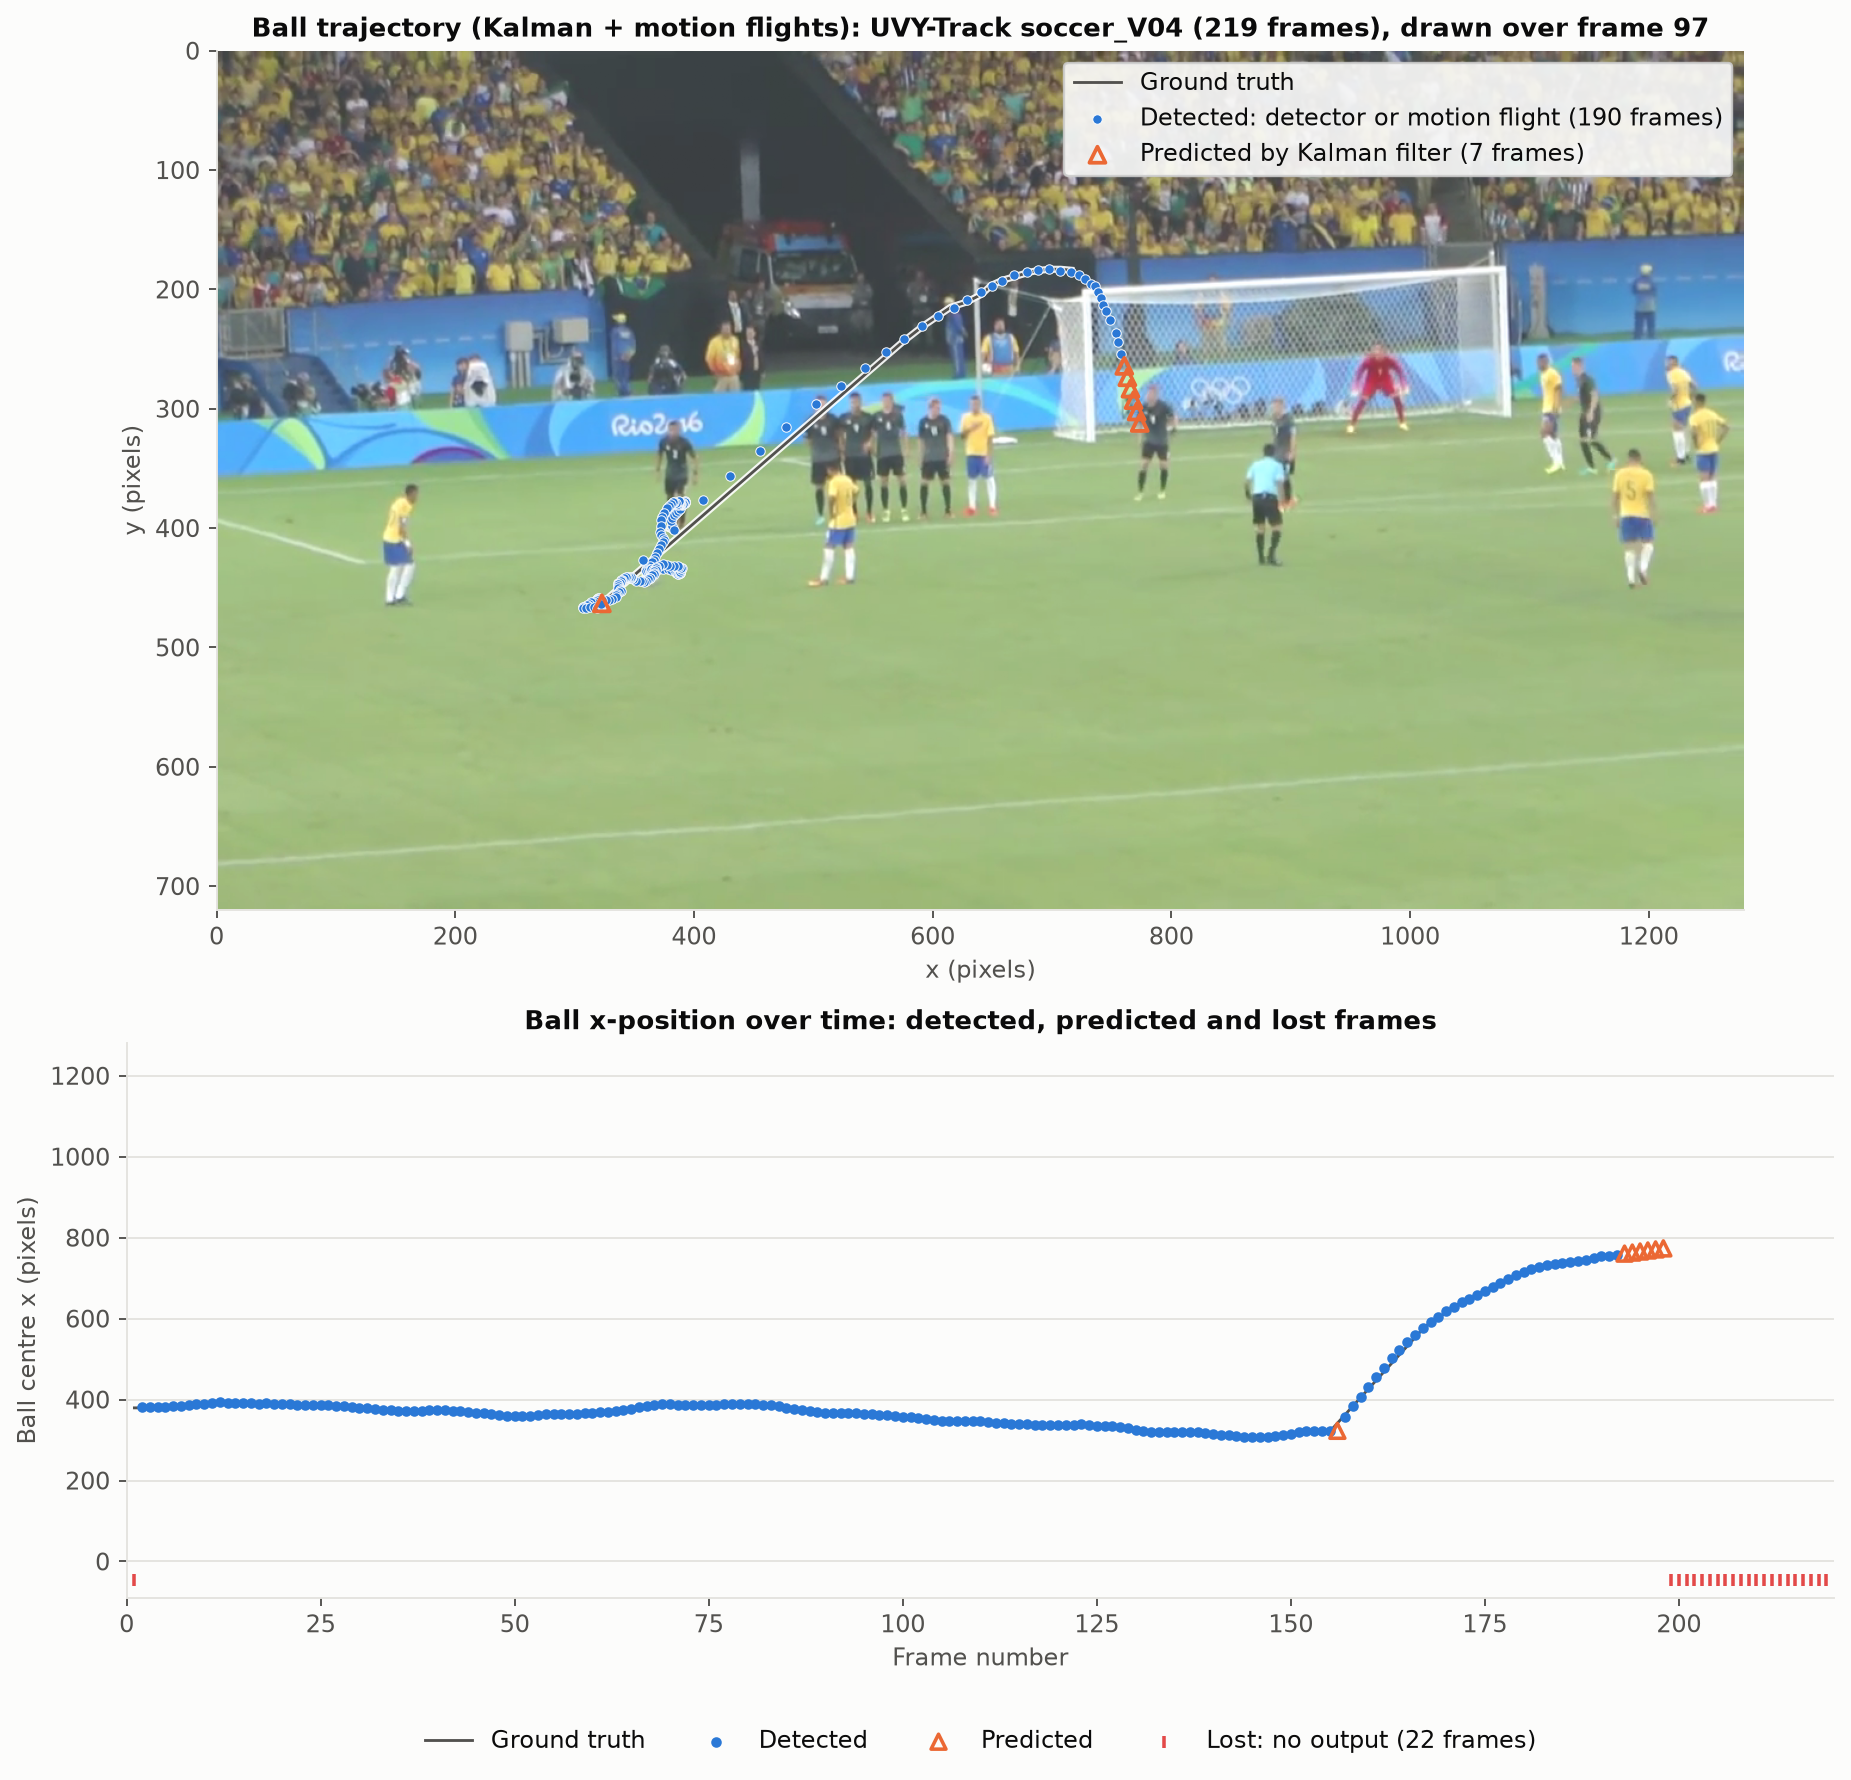
\includegraphics[width=\columnwidth]{fig_ball_trajectory.png}
\caption{Ball trajectory of the proposed tracker on the free kick of
\texttt{soccer\_V04} with ground truth. Dots: detected, by the detector or by a
motion flight. Triangles: predicted by the Kalman filter. Marks on the time axis:
frames without output. The arc is the shot, followed by a motion flight; the
ground truth has a gap during the most blurred part of the flight.}
\label{fig:balltraj}
\end{figure}

\begin{figure}[t]
\centering
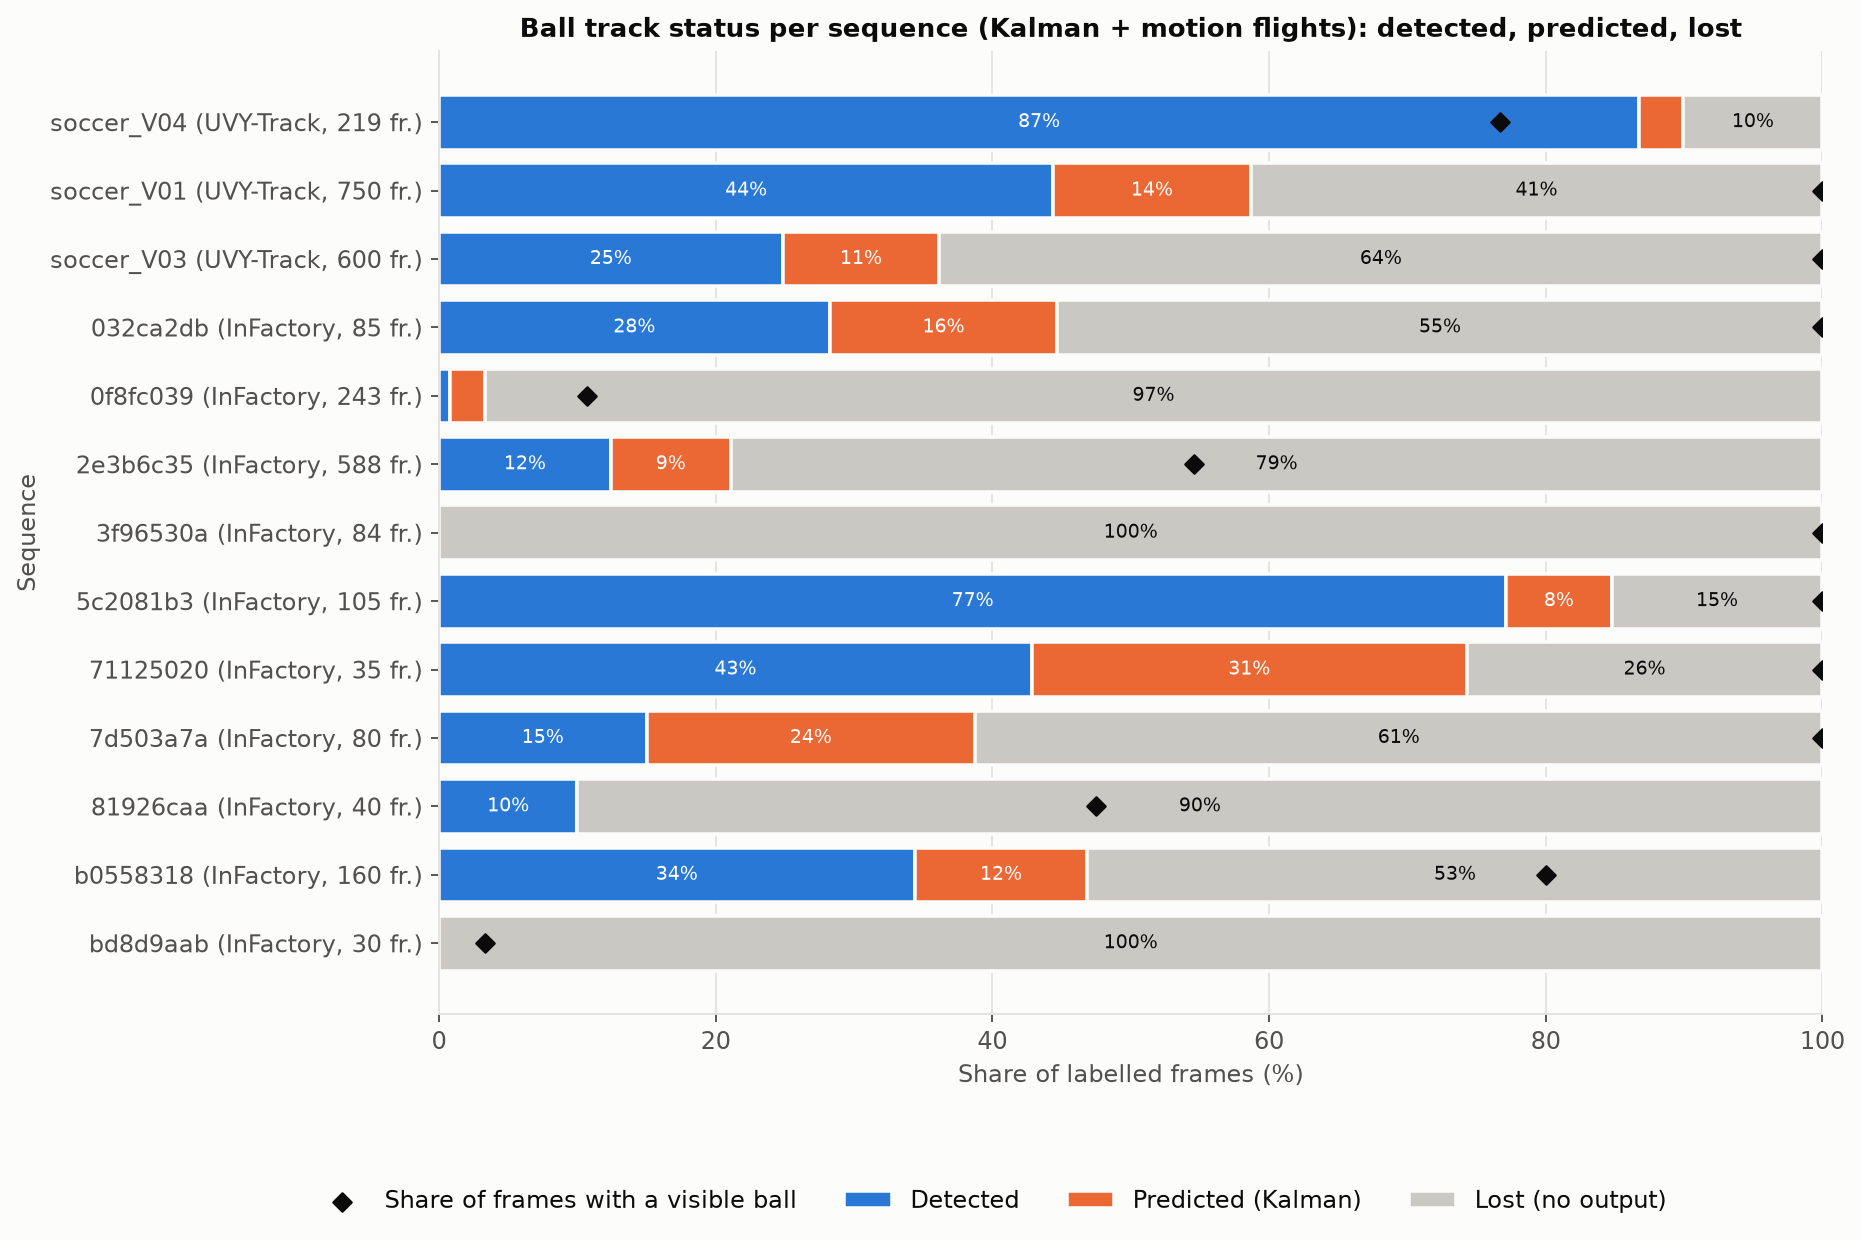
\includegraphics[width=\columnwidth]{fig_ball_status.png}
\caption{Ball track status per sequence with the proposed tracker. Diamonds mark
the share of frames in which the ball is visible.}
\label{fig:ballstatus}
\end{figure}

\subsection{Detector Comparison}
As a secondary experiment, YOLOv8n and YOLO11n were compared with identical
settings on the first 200 frames of one SportsMOT sequence (players) and on two
InFactory clips (ball). Speed was measured by alternating the two models frame by
frame so that both saw the same machine state (Table~\ref{tab:models}). On this
subset YOLO11n is clearly better for players (F1 of 81.2\% against 71.7\%),
mainly through higher precision, and about 5\% faster. For the ball the two
models are practically equal. The two ball clips are among the easier ones, so
their ball scores are above the averages of Table~\ref{tab:ball}. This supports
the choice of YOLO11n but is a small-sample comparison.

\begin{table}[t]
\caption{YOLOv8n Versus YOLO11n on the Same Frames}
\label{tab:models}
\centering
\footnotesize
\setlength{\tabcolsep}{3.5pt}
\begin{adjustbox}{max width=\columnwidth}
\begin{tabular}{@{}llrrrrrr@{}}
\toprule
Model & Target & Frames & Prec. & Rec. & F1 & AP@0.5 & ms/fr. \\
\midrule
YOLOv8n & player & 200 & 60.9 & 87.1 & 71.7 & 71.7 & 112 \\
YOLOv8n & ball & 265 & 83.0 & 67.0 & 74.1 & 51.0 & 112 \\
YOLO11n & player & 200 & 74.5 & 89.2 & 81.2 & 79.0 & 106 \\
YOLO11n & ball & 265 & 88.8 & 64.8 & 74.9 & 51.2 & 106 \\
\bottomrule
\end{tabular}
\end{adjustbox}
\end{table}

\subsection{Runtime}
Table~\ref{tab:runtime} and Fig.~\ref{fig:runtime} give the median time per
frame of every stage, measured over 150 frames of a $1280\times720$ sequence on
an idle machine on mains power. The detector takes 64\% of the time and the ball
motion stage (feature-based frame alignment, differencing and flight linking)
another 30\%. The player trackers cost about a millisecond, so the choice of
tracker changes throughput by under 1\%: the full pipeline runs at 5.68 frames per second with
ByteTrack, 5.68 with SORT and 5.65 with OC-SORT. SORT is the
cheapest tracker, ByteTrack costs slightly more for its second association stage,
and OC-SORT is two to three times slower than both. The system is therefore an
offline analysis tool on this hardware; disabling motion flights removes the
motion stage. Power state matters: on battery the processor is throttled and every
timing changes by a large factor, so the power source is recorded with the results.

\begin{table}[t]
\caption{Median Processing Time per Frame}
\label{tab:runtime}
\centering
\footnotesize
\begin{adjustbox}{max width=\columnwidth}
\begin{tabular}{@{}lrr@{}}
\toprule
Stage & Time (ms) & Share (\%) \\
\midrule
Detection & 112.63 & 64.0 \\
Ball motion: camera compensation + flight linking & 52.83 & 30.0 \\
Video encoding & 4.45 & 2.5 \\
Frame reading & 4.32 & 2.5 \\
Drawing annotations & 1.11 & 0.6 \\
Player filter + ByteTrack & 0.71 & 0.4 \\
Ball filter + Kalman tracker & 0.03 & 0.0 \\
\midrule
\textbf{Total (proposed pipeline)} & \textbf{176.1} & 100.0 \\
\midrule
Player filter + SORT (baseline) & 0.61 & -- \\
Player filter + OC-SORT (baseline) & 1.59 & -- \\
\bottomrule
\end{tabular}
\end{adjustbox}
\end{table}

\begin{figure*}[t]
\centering
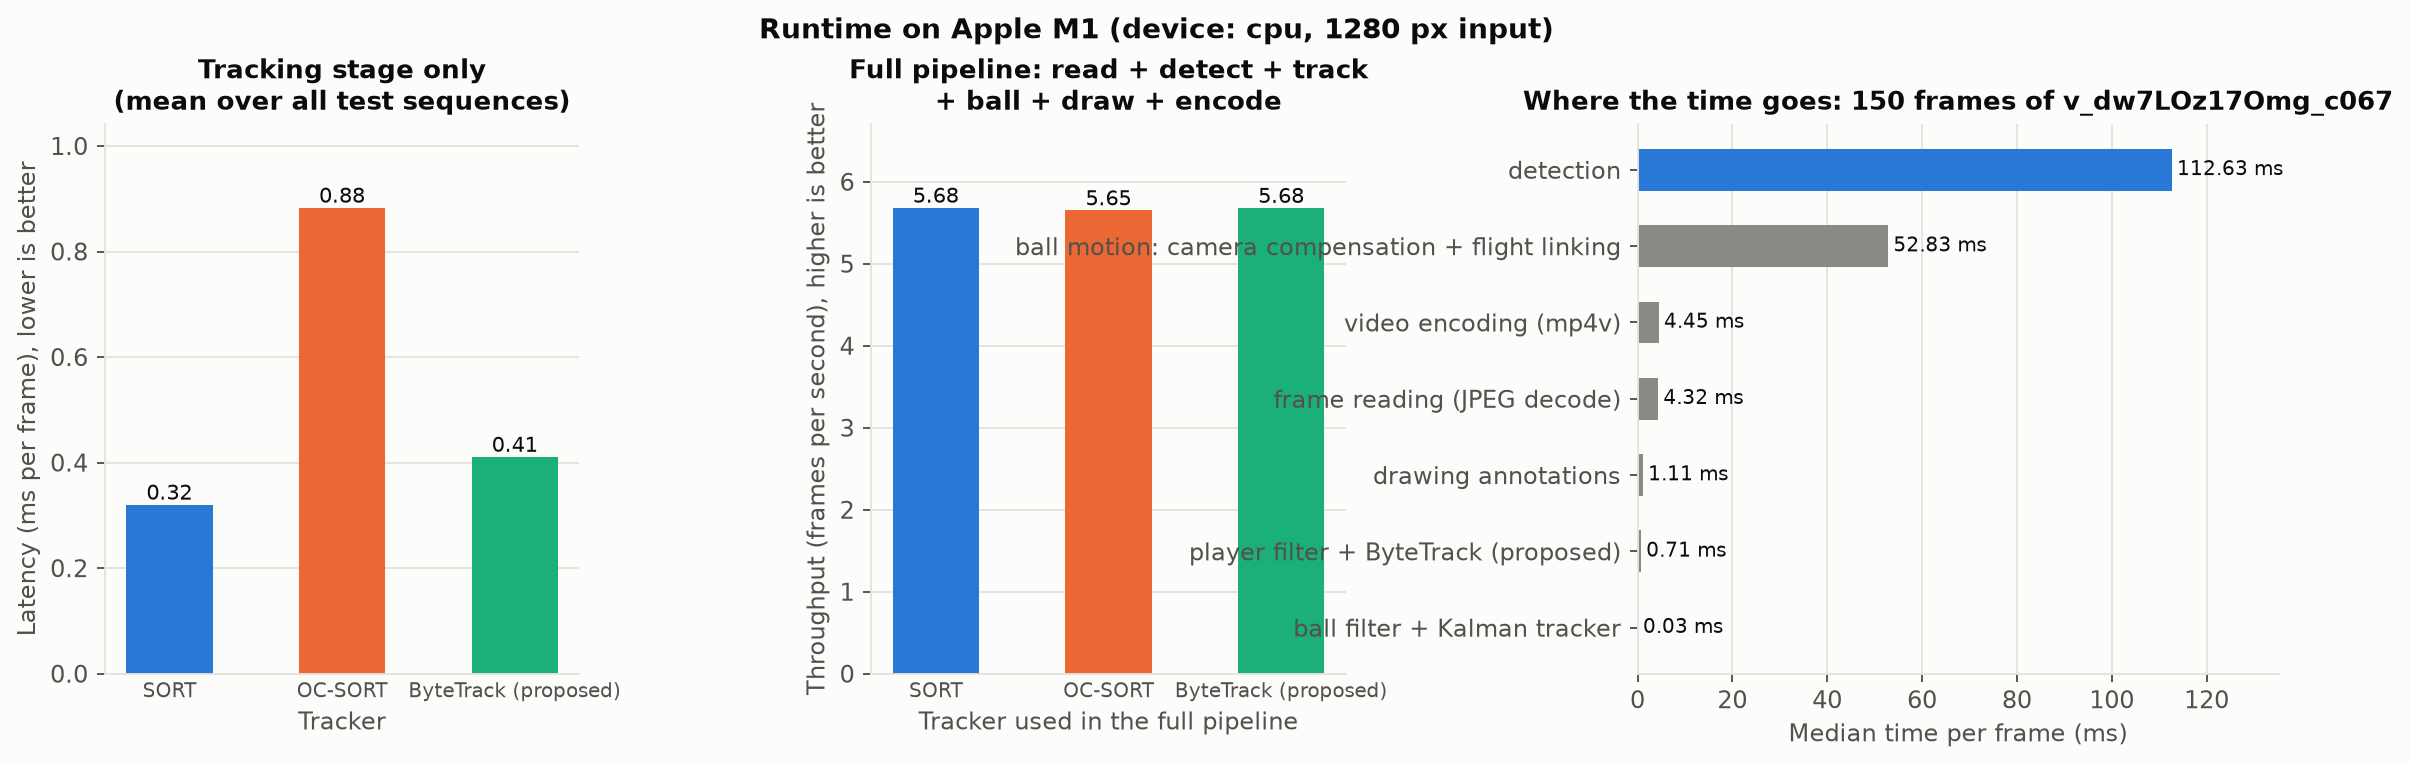
\includegraphics[width=\textwidth]{fig_runtime.png}
\caption{Runtime. Left: latency of the tracking stage alone. Centre: throughput
of the full pipeline. Right: time per stage of the proposed system.}
\label{fig:runtime}
\end{figure*}

\subsection{Qualitative Results}
The application was run end to end on the UVY-Track clip \texttt{soccer\_V04}
(241 frames, a free kick and a goal). It processed the clip in 46 seconds (5.2
frames per second), produced 33 player track identities with a median track
length of 209 frames, and reported the ball in 197 frames, of which 190 were
detected (by the detector or a motion flight) and 7 predicted; the shot is
followed into the net. On a further, previously unseen fan-filmed penalty
shoot-out (\texttt{soccer\_V02}, 1,085 frames) a penalty is likewise followed from
the spot past the diving goalkeeper into the net. Fig.~\ref{fig:demo} shows a frame of the annotated
output. Figs.~\ref{fig:trajectories} and~\ref{fig:heatmap} show player
trajectories and a position heatmap for a SportsMOT sequence; both are in image
coordinates, so camera motion is not compensated.

\begin{figure}[t]
\centering
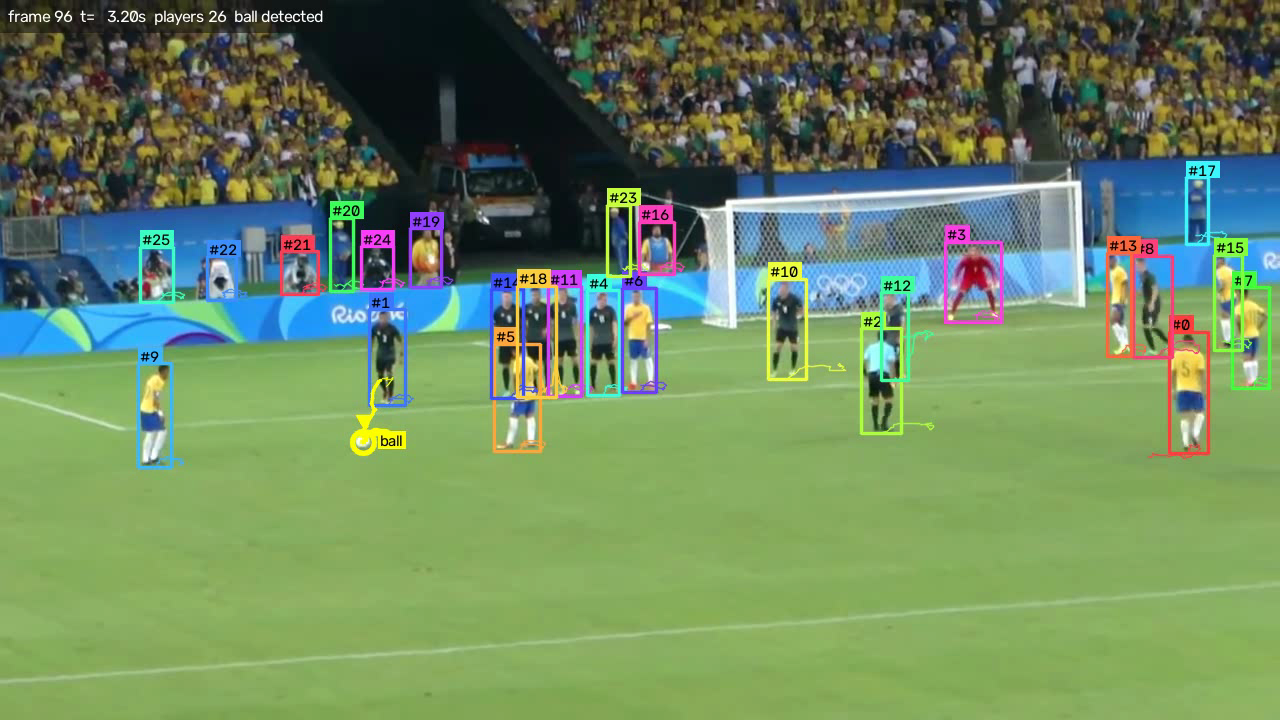
\includegraphics[width=\columnwidth]{fig_demo_screenshot.png}
\caption{A frame of the annotated output video: player boxes with identities and
trails, the ball marker with its recent path, and the status line.}
\label{fig:demo}
\end{figure}

\begin{figure}[t]
\centering
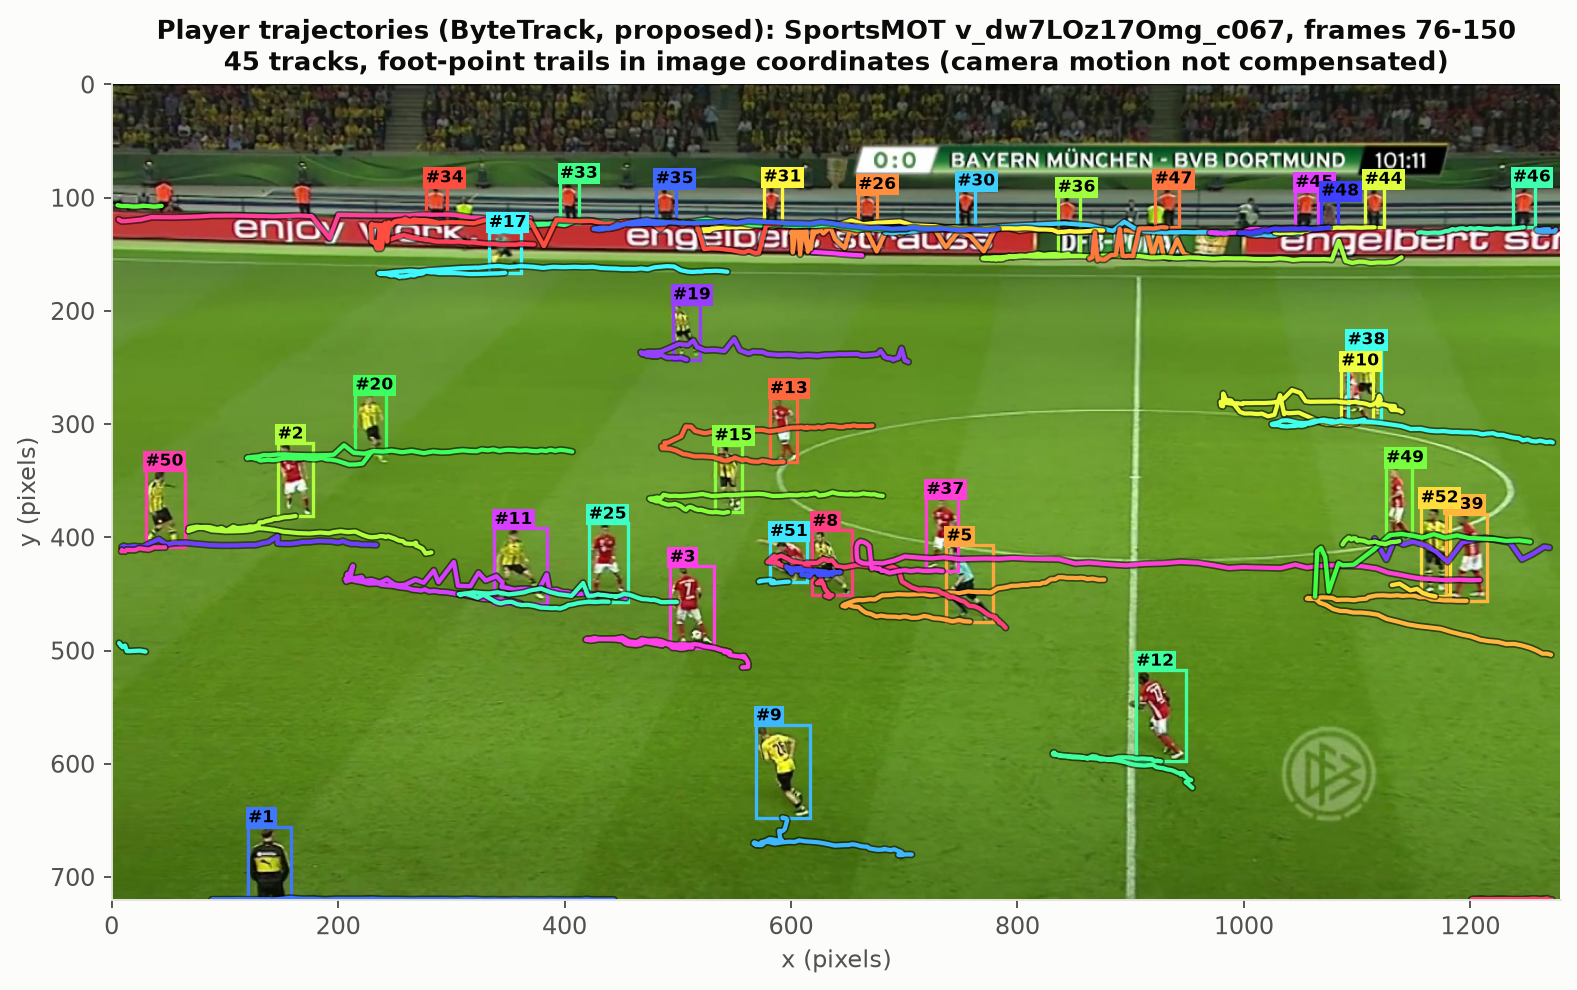
\includegraphics[width=\columnwidth]{fig_player_trajectories.png}
\caption{Player trajectories from ByteTrack over 75 frames of a SportsMOT test
sequence (foot points, image coordinates). The tracks along the top are
perimeter staff, who are detected and tracked but are not annotated in the
benchmark.}
\label{fig:trajectories}
\end{figure}

\begin{figure}[t]
\centering
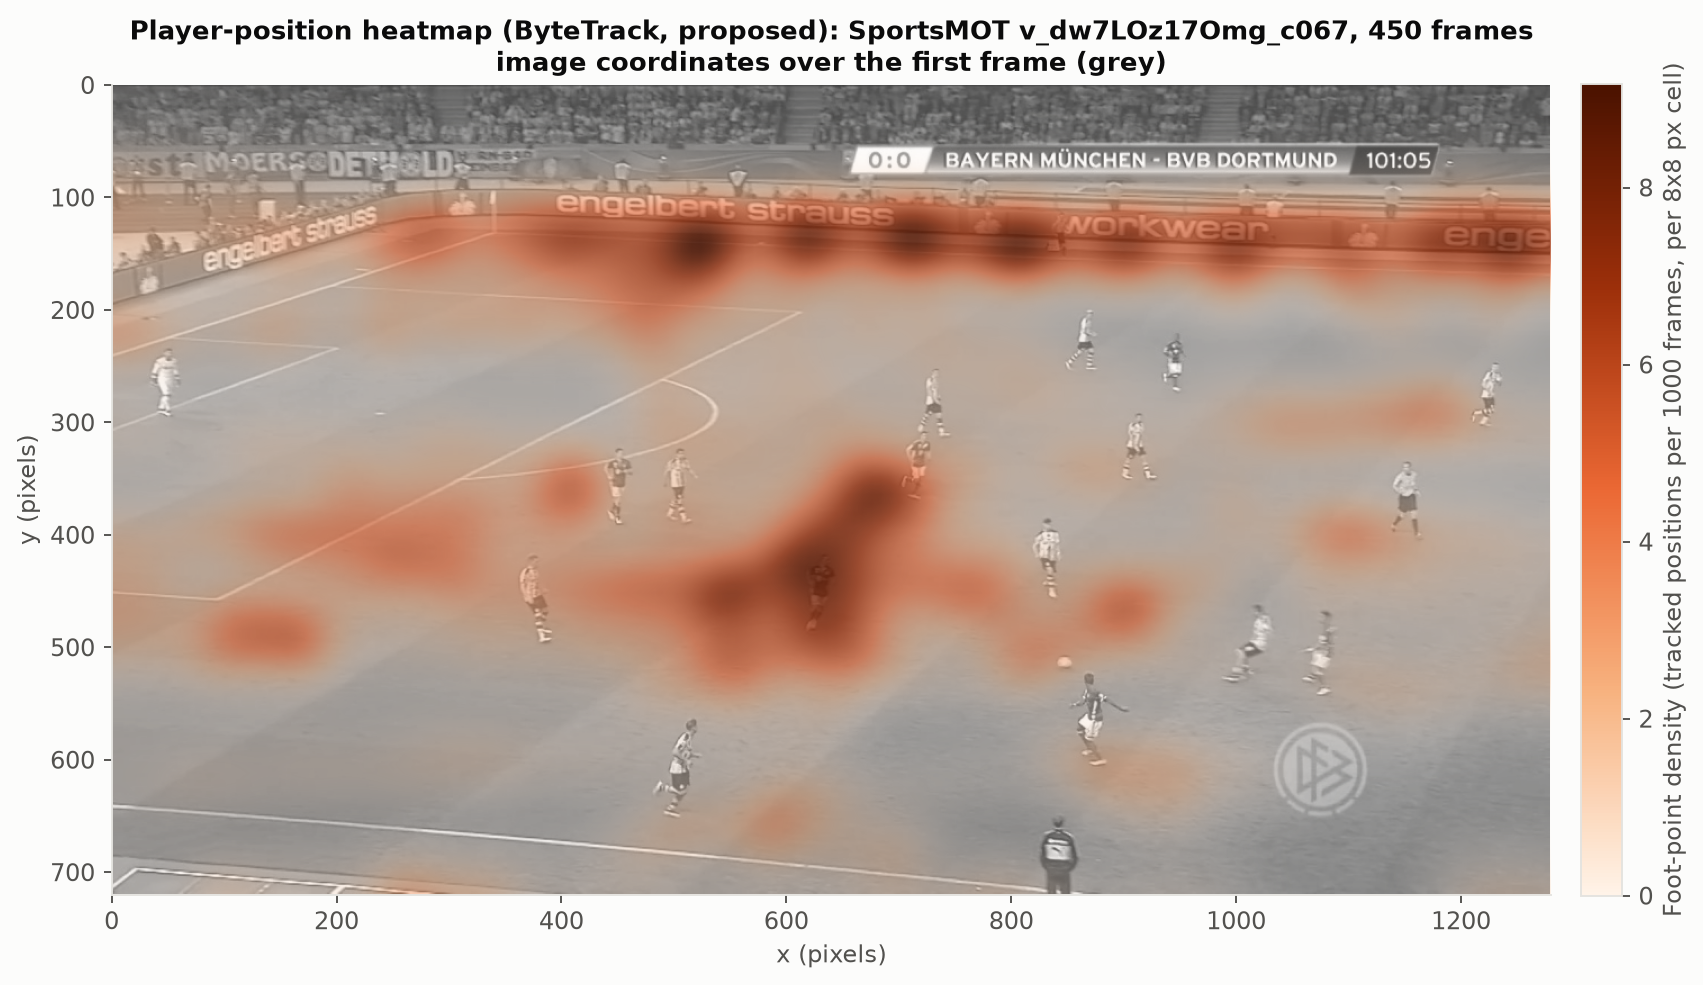
\includegraphics[width=\columnwidth]{fig_player_heatmap.png}
\caption{Player-position heatmap over the same sequence (image coordinates).}
\label{fig:heatmap}
\end{figure}

% =============================================================================
\section{Limitations}
% =============================================================================
\begin{itemize}
\item \emph{Generic detector.} The \emph{person} class also responds to referees,
coaches, staff and spectators, and the \emph{sports ball} class misses most small
broadcast balls. This limits every number in this paper more than the choice of
tracker does.
\item \emph{The proposed tracker is not uniformly best.} ByteTrack gives the most
stable identities and the highest recall, but tuned SORT has a higher HOTA, MOTA
and IDF1 on SportsMOT in this setting.
\item \emph{Small evaluation.} Six tracking test sequences, thirteen ball
sequences and a single tuning sequence; no confidence intervals are given and the
results are not comparable with published leaderboards.
\item \emph{Partial labels.} No single dataset evaluates the whole system:
SportsMOT has no ball labels, UVY-Track labels only part of the people, and
InFactory has neither player labels nor ball identities.
\item \emph{Ball predictions.} A constant-velocity model cannot follow a direction
change; 40\% of the predicted positions are wrong, and the tracker sometimes
follows a false positive or a second real ball beside the pitch.
\item \emph{Motion flights are narrow.} They help only when the ball is struck and
visible in flight, must start where the detector last saw the ball, and are
switched off when the global camera model fails (cuts, dissolves, fast zoom).
Their rules were developed on UVY-Track and refined after a first InFactory run,
because no separate ball tuning set was available.
\item \emph{Scope.} There is no camera-motion compensation for the players,
re-identification, team assignment or pitch calibration, and throughput is about
six frames per second on an Apple M1 processor.
\end{itemize}

% =============================================================================
\section{Future Work}
% =============================================================================
The most valuable next step is a soccer-specific detector with separate classes
for players, referees, goalkeepers and the ball, which addresses the dominant
error source for both players and ball. Tiled high-resolution inference for the
ball is already supported by the application but has not been evaluated. The
ball motion model can be improved with a gravity-aware model for flights and
offline forward-backward smoothing, and motion flights should be evaluated on a
dedicated, fully labelled ball tuning and test split. Camera-motion compensation and appearance-based
re-identification, as in BoT-SORT~\cite{botsort}, would steady trajectories and
identities. Further steps are team assignment from jersey colour, pitch
calibration for positions in metres, accelerated inference for real-time
throughput, and evaluation on the complete validation splits with several tuning
sequences.

% =============================================================================
\section{Conclusion}
% =============================================================================
A complete player-and-ball tracking system was built, tested and evaluated on
three public datasets with a reproducible protocol. With identical detections,
ByteTrack produced the fewest identity switches and the highest recall on both
tracking datasets and the best OWTA on UVY-Track, while tuned SORT obtained the
best HOTA, MOTA and IDF1 on SportsMOT; OC-SORT was the weakest in association and
the slowest. The dedicated Kalman ball tracker improved ball precision, F1 and
above all the continuity of the ball track over detection alone, and motion-based
flights let it follow a struck ball that the detector loses without changing the
result on clips without such a shot. Its predicted positions are still wrong 40\%
of the time, which justifies labelling them separately. Across all experiments the generic lightweight detector, not the
tracker, limits both accuracy and speed, so a soccer-specific detector is the
most promising improvement.

% =============================================================================
\begin{thebibliography}{00}
\bibitem{sort} A. Bewley, Z. Ge, L. Ott, F. Ramos, and B. Upcroft, ``Simple online and realtime tracking,'' in \emph{Proc. IEEE Int. Conf. Image Process. (ICIP)}, 2016, pp. 3464--3468.
\bibitem{deepsort} N. Wojke, A. Bewley, and D. Paulus, ``Simple online and realtime tracking with a deep association metric,'' in \emph{Proc. IEEE Int. Conf. Image Process. (ICIP)}, 2017, pp. 3645--3649.
\bibitem{bytetrack} Y. Zhang, P. Sun, Y. Jiang, D. Yu, F. Weng, Z. Yuan, P. Luo, W. Liu, and X. Wang, ``ByteTrack: Multi-object tracking by associating every detection box,'' in \emph{Proc. Eur. Conf. Comput. Vis. (ECCV)}, 2022.
\bibitem{ocsort} J. Cao, J. Pang, X. Weng, R. Khirodkar, and K. Kitani, ``Observation-centric SORT: Rethinking SORT for robust multi-object tracking,'' in \emph{Proc. IEEE/CVF Conf. Comput. Vis. Pattern Recognit. (CVPR)}, 2023.
\bibitem{botsort} N. Aharon, R. Orfaig, and B.-Z. Bobrovsky, ``BoT-SORT: Robust associations multi-pedestrian tracking,'' arXiv:2206.14651, 2022.
\bibitem{yolo} J. Redmon, S. Divvala, R. Girshick, and A. Farhadi, ``You only look once: Unified, real-time object detection,'' in \emph{Proc. IEEE Conf. Comput. Vis. Pattern Recognit. (CVPR)}, 2016, pp. 779--788.
\bibitem{yolo11} G. Jocher and J. Qiu, ``Ultralytics YOLO11,'' software, 2024. [Online]. Available: \url{https://github.com/ultralytics/ultralytics}
\bibitem{coco} T.-Y. Lin, M. Maire, S. Belongie, J. Hays, P. Perona, D. Ramanan, P. Doll\'ar, and C. L. Zitnick, ``Microsoft COCO: Common objects in context,'' in \emph{Proc. Eur. Conf. Comput. Vis. (ECCV)}, 2014, pp. 740--755.
\bibitem{sportsmot} Y. Cui, C. Zeng, X. Zhao, Y. Yang, G. Wu, and L. Wang, ``SportsMOT: A large multi-object tracking dataset in multiple sports scenes,'' in \emph{Proc. IEEE/CVF Int. Conf. Comput. Vis. (ICCV)}, 2023.
\bibitem{soccernet} A. Cioppa, S. Giancola, A. Deli\`ege, L. Kang, X. Zhou, Z. Cheng, B. Ghanem, and M. Van Droogenbroeck, ``SoccerNet-Tracking: Multiple object tracking dataset and benchmark in soccer videos,'' in \emph{Proc. IEEE/CVF Conf. Comput. Vis. Pattern Recognit. Workshops (CVPRW)}, 2022, pp. 3491--3502.
\bibitem{uvy} E. Alencar and R. de Freitas, ``UVY: A dataset of sport user-generated videos from YouTube for multi-object tracking evaluation,'' Zenodo, 2026. [Online]. Available: \url{https://zenodo.org/records/21303900}
\bibitem{uvypaper} E. Alencar, L. Pessoa, F. Costa, G. Souza, and R. de Freitas, ``Comparative analysis of deep learning-based multi-object tracking approaches applied to sports user-generated videos,'' in \emph{Proc. 20th Int. Joint Conf. Comput. Vis., Imag. Comput. Graph. Theory Appl. (VISAPP)}, 2025, pp. 691--698.
\bibitem{infactory} V. Constantinou, M. Iranmanesh, and J. Kanalakis, ``Soccer ball tracking dataset,'' Infactory, 2026. [Online]. Available: \url{https://huggingface.co/datasets/infactory-ai/ball-tracking}
\bibitem{kalman} R. E. Kalman, ``A new approach to linear filtering and prediction problems,'' \emph{J. Basic Eng.}, vol. 82, no. 1, pp. 35--45, 1960.
\bibitem{hungarian} H. W. Kuhn, ``The Hungarian method for the assignment problem,'' \emph{Naval Res. Logist. Quart.}, vol. 2, no. 1--2, pp. 83--97, 1955.
\bibitem{deepball} J. Komorowski, G. Kurzejamski, and G. Sarwas, ``DeepBall: Deep neural-network ball detector,'' in \emph{Proc. Int. Conf. Comput. Vis. Theory Appl. (VISAPP)}, 2019.
\bibitem{tracknet} Y.-C. Huang, I.-N. Liao, C.-H. Chen, T.-U. Ik, and W.-C. Peng, ``TrackNet: A deep learning network for tracking high-speed and tiny objects in sports applications,'' in \emph{Proc. IEEE Int. Conf. Adv. Video Signal Based Surveill. (AVSS)}, 2019.
\bibitem{soccertrack} A. Scott, I. Uchida, M. Onishi, Y. Kameda, K. Fukui, and K. Fujii, ``SoccerTrack: A dataset and tracking algorithm for soccer with fish-eye and drone videos,'' in \emph{Proc. IEEE/CVF Conf. Comput. Vis. Pattern Recognit. Workshops (CVPRW)}, 2022, pp. 3569--3579.
\bibitem{teamtrack} A. Scott \emph{et al.}, ``TeamTrack: A dataset for multi-sport multi-object tracking in full-pitch videos,'' arXiv:2404.13868, 2024.
\bibitem{survey} M. Manafifard, H. Ebadi, and H. Abrishami Moghaddam, ``A survey on player tracking in soccer videos,'' \emph{Comput. Vis. Image Understand.}, vol. 159, pp. 19--46, 2017.
\bibitem{sahi} F. C. Akyon, S. O. Altinuc, and A. Temizel, ``Slicing aided hyper inference and fine-tuning for small object detection,'' in \emph{Proc. IEEE Int. Conf. Image Process. (ICIP)}, 2022.
\bibitem{hota} J. Luiten, A. O\v{s}ep, P. Dendorfer, P. Torr, A. Geiger, L. Leal-Taix\'e, and B. Leibe, ``HOTA: A higher order metric for evaluating multi-object tracking,'' \emph{Int. J. Comput. Vis.}, vol. 129, 2021.
\bibitem{clear} K. Bernardin and R. Stiefelhagen, ``Evaluating multiple object tracking performance: The CLEAR MOT metrics,'' \emph{EURASIP J. Image Video Process.}, 2008.
\bibitem{idf1} E. Ristani, F. Solera, R. Zou, R. Cucchiara, and C. Tomasi, ``Performance measures and a data set for multi-target, multi-camera tracking,'' in \emph{Proc. Eur. Conf. Comput. Vis. Workshops (ECCVW)}, 2016.
\bibitem{trackers} Roboflow, ``trackers,'' software, version 2.6.1, 2026. [Online]. Available: \url{https://github.com/roboflow/trackers}
\bibitem{trackeval} J. Luiten and A. Hoffhues, ``TrackEval,'' software, 2020. [Online]. Available: \url{https://github.com/JonathonLuiten/TrackEval}
\bibitem{yu2006} X. Yu, H. W. Leong, C. Xu, and Q. Tian, ``Trajectory-based ball detection and tracking in broadcast soccer video,'' \emph{IEEE Trans. Multimedia}, vol. 8, no. 6, 2006.
\bibitem{orb} E. Rublee, V. Rabaud, K. Konolige, and G. Bradski, ``ORB: An efficient alternative to SIFT or SURF,'' in \emph{Proc. IEEE Int. Conf. Comput. Vis. (ICCV)}, 2011.
\bibitem{ransac} M. A. Fischler and R. C. Bolles, ``Random sample consensus: A paradigm for model fitting with applications to image analysis and automated cartography,'' \emph{Commun. ACM}, vol. 24, no. 6, 1981.
\bibitem{owta} Y. Liu, I. E. Zulfikar, J. Luiten, A. Dave, D. Ramanan, B. Leibe, A. O\v{s}ep, and L. Leal-Taix\'e, ``Opening up open world tracking,'' in \emph{Proc. IEEE/CVF Conf. Comput. Vis. Pattern Recognit. (CVPR)}, 2022.
\end{thebibliography}

\end{document}
